%%%%%%%%%%%%%%%%%%%%%%%%%%%%%%%%%%%%%%%%%%%%%%%%%%%%%%%%%%%%%%%%%%%%%%%%%%%%%
%%%% Preamble
%%%%%%%%%%%%%%%%%%%%%%%%%%%%%%%%%%%%%%%%%%%%%%%%%%%%%%%%%%%%%%%%%%%%%%%%%%%%%

%%%% The uwthesis.sty file relies on the memoir class!
%%%% You should be using the memoir class anyway; it makes life easier:
%%%% http://www.ctan.org/tex-archive/macros/latex/contrib/memoir/
\documentclass[oneside, letterpaper, 12pt, oldfontcommands]{memoir}

%%%% Import uwthesis.sty to get official formatting, then set your variables.
\usepackage{uwthesis}
\usepackage{hyperref}
\usepackage{cite}
\usepackage{graphicx}
\usepackage{siunitx}
\usepackage{fontspec}
\usepackage{amssymb}
\newcommand{\fbinv}{\ensuremath{fb^{-1}}}

\newcommand{\PZ}{\ensuremath{Z}}
\newcommand{\Pgamma}{\ensuremath{\gamma}}
\newcommand{\Pn}{\ensuremath{\nu}}
\newcommand{\Pan}{\ensuremath{\bar{\Pn}}}
\newcommand{\zinvg}{\ensuremath{\PZ(\Pn\Pan)\Pgamma}}

\newcommand{\PW}{\ensuremath{W}}
\newcommand{\PWplus}{\ensuremath{W^\mathrm{+}}}
\newcommand{\PWminus}{\ensuremath{W^\mathrm{-}}}
\newcommand{\PWone}{\ensuremath{W^{1}}}
\newcommand{\PWtwo}{\ensuremath{W^{2}}}
\newcommand{\PWthree}{\ensuremath{W^{3}}}
\newcommand{\PB}{\ensuremath{B}}
\newcommand{\Pg}{\ensuremath{g}}
\newcommand{\PH}{\ensuremath{H}}
\newcommand{\Pp}{\ensuremath{p}}
\newcommand{\Pq}{\ensuremath{q}}
\newcommand{\Paq}{\ensuremath{\bar{q}}}
\newcommand{\Pu}{\ensuremath{u}}
\newcommand{\Pd}{\ensuremath{d}}
\newcommand{\Pc}{\ensuremath{c}}
\newcommand{\Ps}{\ensuremath{s}}
\newcommand{\Pt}{\ensuremath{t}}
\newcommand{\Pb}{\ensuremath{b}}
\newcommand{\Pe}{\ensuremath{e}}
\newcommand{\Pmu}{\ensuremath{\mu}}
\newcommand{\Ptau}{\ensuremath{\tau}}
\newcommand{\Pne}{\ensuremath{\Pn_\mathrm{e}}}
\newcommand{\Pnmu}{\ensuremath{\Pn_\mathrm{\mu}}}
\newcommand{\Pntau}{\ensuremath{\Pn_\mathrm{\tau}}}

\newcommand{\pT}{\ensuremath{p_\mathrm{T}}}
\newcommand{\vecpT}{\ensuremath{\vec{p}_\mathrm{T}}}
\newcommand{\ET}{\ensuremath{E_\mathrm{T}}}
\newcommand{\ETgamma}{\ensuremath{E_\mathrm{T}^{\gamma}}}
\newcommand{\MT}{\ensuremath{M_\mathrm{T}}}
\newcommand{\MET}{\ensuremath{p_\mathrm{T}^\mathrm{miss}}}
\newcommand{\vecMET}{\ensuremath{\vec{p}_\mathrm{T}^\mathrm{miss}}}

% Hyphenation of uncommon terms
\hyphenation{cal-ori-me-ter}
\hyphenation{cal-ori-me-ters}

\setsecnumdepth{subsection}

\settitle{A Measurement of \zinvg\ Production and a Search for New Physics in
Monophoton Events Using the CMS Detector at the LHC}
\setauthor{James Joseph Buchanan}
\setdepartment{Physics}
\doctors % or \masters
\setgraddate{201X}
\setdefensedate{T.B.D.} % or whatever format you want

%%%% Members of the Final Oral Committee (FOC)
%%%% Give name, rank, and department
%%%% 
\setfoca{Sridhara Dasu}{Professor}{Physics} % <- Your advisor
\setfocb{Wesley Smith}{Emeritus Professor}{Physics}
\setfocc{Matthew Herndon}{Professor}{Physics}
\setfocd{T.B.D.}{Professor}{Physics}
\setfoce{T.B.D.}{Professor}{T.B.D.}
% \setfocf{Grover Cleveland}{Professor}{Zoology}

%%%% Your abstract, used for the UMI abstract and in your front matter
\setabstract{%
  This thesis presents several studies of monophoton final states
  using 35.9 \fbinv\ of 13\unit{TeV} proton--proton collision data collected by the CMS
  experiment at the LHC in 2016. The standard model \zinvg\ cross section is measured
  as a function of photon transverse momentum. No significant deviations from standard
  model predictions are observed.
  The results are also interpreted in the context of several new physics models.
  Limits are placed on coupling strengths of anomalous triple gauge couplings between
  photons and \PZ\ bosons,
  new particle masses in simplified models of dark matter, the suppression scale of a dark matter
  effective field theory model, and the graviton mass scale in a model of extra
  spatial dimensions.
}

%%%%%%%%%%%%%%%%%%%%%%%%%%%%%%%%%%%%%%%%%%%%%%%%%%%%%%%%%%%%%%%%%%%%%%%%%%%%%
%%%% Document
%%%%%%%%%%%%%%%%%%%%%%%%%%%%%%%%%%%%%%%%%%%%%%%%%%%%%%%%%%%%%%%%%%%%%%%%%%%%%

\begin{document}

% Tell the memoir class to set up lowercase roman for pagination, etc.
\frontmatter

%%%% Uncomment this to create a UMI abstract page.
%%%% If you are submitting electronically, however, this page is unnecessary.
% \theumiabstract

% The title page
\thetitlepage
\clearpage

% The copyright page, if you want to pay the fee and register copyright.
\thecopyrightpage
\cleardoublepage

% These above pages should not be counted, so we reset the counter to 1.
\setcounter{page}{1}

% An abstract may be required by your department.
\section{Abstract}
\uwabstract
\cleardoublepage

% Acknowledgements go here if you want to include them.
% \section{Acknowledgements}
% This document would never have come to fruition without the support of my colleagues
% and friends in the UW-Madison CMS group.
% Wesley Smith, Sridhara Dasu, and Matt Herndon are great physicists and leaders
% who have nurtured a rigorous standard of excellence that this group
% can rightly be proud of.
% Bhawna Gomber's deep expertise, organizational acumen,
% and untiring work ethic have pushed these analyses forward at every step. These
% results are as much hers as they are mine.
% Tom Perry helped to develop a previous iteration of these analyses,
% and freely contributed his assistance and code to let us hit the ground running in 2016.
% Devin Taylor, Tyler Ruggles, Nate Woods, Laura Dodd, Kenneth Long, and
% Usama Hussein were all top-notch office mates, whose insights I've taken advantage of
% on countless occasions.
% Special recognition goes to Nick Smith, whose encyclopedic thesis served as an excellent reference
% for this one.
% I must finally thank my parents, Yvonne and Darryl Buchanan,
% for their perpetual support of everything I do.
% \clearpage

% Table of contents
\maxtocdepth{subsection}
\tableofcontents* % the * means that there isn't an entry for the TOC itself
% \clearpage
% \listoffigures  % if you have any figures
% \clearpage
% \listoftables   % if you have any tables

% Tell the memoir class to set up normal pagination, etc. for the main doc
\mainmatter

\chapter{Introduction} \label{chap:introduction}
\section{Overview} \label{sec:introduction_overview}
This thesis presents several analyses of event
yields in ``monophoton'' final states, characterized by a single \Pgamma\ with high transverse
momentum, along with an overall transverse momentum imbalance typically of equal magnitude and opposite direction to
that of the photon.
These analyses correspond to 35.9 \fbinv\ of 13\unit{TeV} proton-proton (\Pp\Pp) collision data collected in 2016 by the CMS
detector at the LHC. A measurement of the production rate for the process $\Pp\Pp \to \PZ\Pgamma \to \Pn\Pan\Pgamma$ is obtained
and compared to predictions derived from the standard model (SM) of particle physics. No significant deviation from SM
predictions is observed.

The predicted monophoton yield in several theories of physics beyond the SM (BSM) is higher than the SM prediction.
This thesis examines two varieties of anomalous triple gauge coupling (aTGC), simplified models of dark matter (DM)
interacting with SM matter via a vector or axial-vector mediator, an effective field theory (EFT) of DM interaction
with  \Pgamma\ and \PZ\ bosons, and a model of extra spatial dimensions. For each of these models, 95\% confidence level (CL)
limits are placed on relevant parameters based on the observed collision data.

\section{Standard model of particle physics} \label{sec:introduction_standard_model}
The \textit{standard model} of particle physics is our current best mathematical framework for describing the behavior
of elementary particles. The set of particles described by the SM is illustrated in Fig.~\ref{fig:sm_particles}, which
groups them according to certain fundamental characteristics.
Each particle has an intrinsic angular momentum known as \text{spin}, specified by the lower number in each square of Fig.~\ref{fig:sm_particles}.
Spin can be an integer or half-integer, according to which the particle is classified as a \textit{boson} or \textit{fermion}, respectively.
The fundamental fermions comprise six ``flavors'' of quarks---up (\Pu), down (\Pd), charm (\Pc), strange (\Ps), top (\Pt), and bottom (\Pb)---and six flavors of
leptons: electron (\Pe), muon (\Pmu), and tau (\Ptau), with three corresponding neutrinos (\Pne, \Pnmu, \Pntau).
Each of these has both a particle and an anti-particle variety; the quarks additionally come in three ``colors''.
We typically denote a particle by a letter, e.g. $q$ for a generic quark; its antiparticle partner has an overbar, e.g. $\bar{q}$.
The fundamental bosons comprise the \PH\ as well as the gauge bosons, in turn comprising the \PZ, photon (\Pgamma),
two \PW s distinguished by their electric charge, and eight gluons (\Pg) distinguished by a color-anticolor doublet.

\begin{figure}[hbtp]
  \begin{center}
    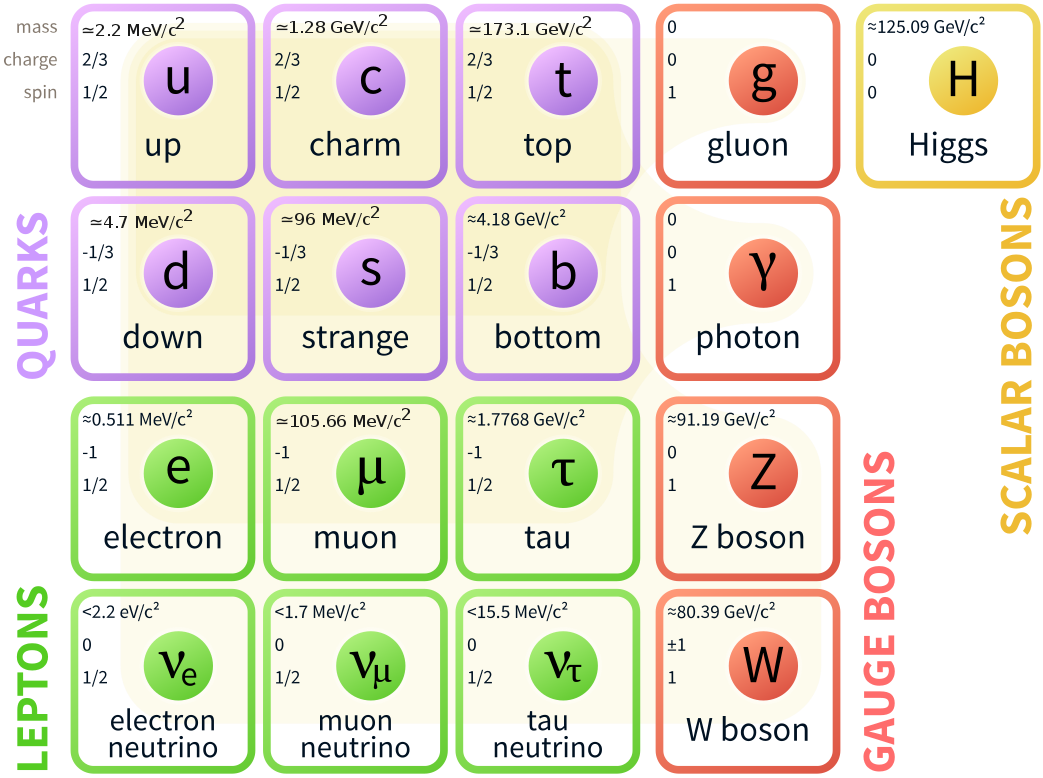
\includegraphics[width=1.0\textwidth]{Figures/sm_particles.png}
    \caption{
      The particles of the Standard Model.
    }
    \label{fig:sm_particles}
  \end{center}
\end{figure}

The particles are related to one another through various
classes of interactions, each of which has a corresponding charge whose sum must be conserved in any physical process.
The electromagnetic and weak interactions correspond to electric charge and weak isospin, respectively.
In Fig.~\ref{fig:sm_particles}, the value $Q$ of the electric charge is specified by the middle number in each square.
For quarks and leptons, weak isospin determines whether the particle is ``up-type''
(\Pu, \Pd, \Pt, \Pne, \Pnmu, \Pntau) or ``down-type'' (\Pd, \Ps, \Pb, \Pe, \Pmu, \Ptau).
Weak isospin has a corresponding value $T_{3}$: up-type fermions have $T_{3} = \mathrm{+}1/2$, down-type fermions and the \PH\ have
$T_{3} = \mathrm{-}1/2$, $W^\pm$ have $T_{3} = \pm1$, and the other bosons have $T_{3} = 0$.
The three colors carried by quarks and gluons are associated with the strong interaction, described by the theory of \textit{quantum
chromodynamics} (QCD). The preceding discussion applies to normal (i.e. not anti-) particles; antiparticles carry opposite values of all the
aforementioned charges.

These interactions lead to the relationships illustrated in Fig.~\ref{fig:sm_interactions}, in which every linkage represents
a direct \textit{coupling}, which allows a particle at one end of the link to evolve directly into a particle at the other end.
Particles with a nonzero electric charge are all coupled directly to the photon. The photon is coupled to the weak bosons
(\PZ\ and \PW), which in turn couple to all of the fundamental fermions.
The gluons couple directly with each other and with the quarks.
Particles that couple directly to the \PH\ have an intrinsic mass (specified by the top number in each square of Fig.~\ref{fig:sm_particles})
tied to the strength of their coupling. In the SM, any particle that does not couple directly to the \PH\ is massless.

\begin{figure}[hbtp]
  \begin{center}
    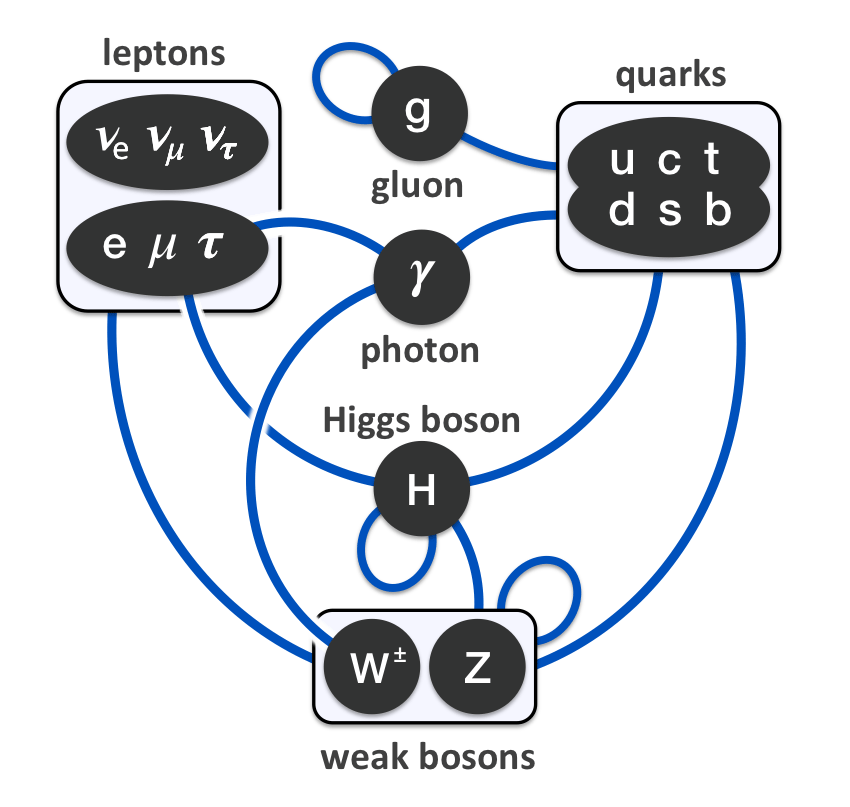
\includegraphics[width=0.7\textwidth]{Figures/Elementary_particle_interactions_in_the_Standard_Model.png}
    \caption{
      Standard Model couplings.
    }
    \label{fig:sm_interactions}
  \end{center}
\end{figure}

The full dynamics of the SM is encapsulated mathematically by a \textit{Lagrangian} function. Particles correspond to operator
terms appearing in the Lagrangian, and a coupling of one particle to another is described by multiplying their
corresponding operators together. The SM Lagrangian is unchanged
if all its fermion operators are multiplied by any complex number of the form $e^{iY\theta}$, where the \textit{hypercharge} $Y$ is a value that depends
on the operator being multiplied. The is true even if $\theta$ is allowed to have different arbitrary values at
different points in space and time, but any operator with a nonzero $Y$ couples to an additional operator denoted by \PB,
and as a consequence the first derivatives of $\theta$ in space and time must also be subtracted from \PB.
This deep level of invariance is called a \textit{gauge symmetry}, with \PB\ the associated \textit{gauge boson}.
Multiplication by $e^{i\theta}$ is characterized by the group $U(1)$, so we say that the SM Lagrangian has a
$U(1)_{Y}$ gauge symmetry associated with the \PB.

In a similar vein, the SM Lagrangian is unchanged if matching doublets
of weak isospin up- and down-type operators are multiplied by unitary $2\times2$ matrices with determinant 1, described by the
group $SU(2)$. Those with a nonzero weak isospin couple to every $W^{i}$ ($i=1,2,3$), which must receive their own balancing transformations
if the fermion $SU(2)$ transformations are allowed to vary as a function of space and time.
Hence we say that the SM Lagrangian has an $SU(2)$ gauge symmetry associated with the gauge bosons $W^{i}$.

The \PB\ and $W^{i}$s also couple to the \PH, and the structure of this coupling constrains the physical states
most easily accessed by these operators, corresponding to four distinct linear combinations of
\PB\ and $W^{i}$. These combinations, which are themselves operators, are labeled \PZ, \Pgamma, \PWplus, and \PWminus,
and these are the operators describing the physical particles detected in experiments.
In this manner, the electromagnetic and weak interactions are intertwined into the \textit{electroweak} (EWK) interaction.
The conserved electric charge $Q$ emerges as the sum of $T_{3}$ with $\frac{1}{2}Y$.

Finally, the SM Lagrangian has an additional $SU(3)$ gauge symmetry associated with the eight gluons and color charge, described by QCD.
Particles with color charge do not exist stably on their own, but rather are always observed in bound states called \textit{hadrons}, in which the overall color
charge state is invariant under any $SU(3)$ transformation. One such ``colorless'' configuration is the proton (\Pp), which
to a first approximation may be thought of as a bound state of two $u$ quarks and one $d$ quark.

However, the mass of the proton is much greater than the sum of the masses of these three components, and this additional mass is associated with an effervescent
``sea'' of \textit{partons}, transient particles swarming the proton that can only be distinguished at high energies.
Known partons include gluons (carrying about 50\% of the total momentum of a high-energy proton),
all types of quark and antiquark, and photons. As a consequence, a high-energy collision between two protons can give rise to a $q\bar{q}$ interaction,
which is the primary catalyst for all the processes studied below. A single parton carries some fraction of the total energy carried by the whole proton,
so in general, partons collide with a lower interaction energy than that of the protons that carry them.
The square of the center-of-mass energy of colliding protons is denoted by $s$, while that of a specific
parton-parton interaction is denoted by $\hat{s}$.

This rapid overview of the SM necessarily elides many essential nuances of the underlying mathematical formalism. These are more fully
documented in numerous comprehensive texts on the subject, e.g.~\cite{ref:HalzenMartin, ref:BargerPhillips, ref:PeskinSchroeder, ref:Srednicki, ref:Schwartz}.

The domain of applicability of the SM is quite substantial, encompassing
every well-measured fundamental interaction of every verified fundamental particle. All SM particles have been conclusively observed,
and no fundamental particles outside the SM have ever been conclusively observed. After decades of effort by thousands of researchers,
no significant deviation from SM predictions has ever been confirmed in high-energy scattering experiments~\cite{ref:PDG}.
These efforts are extended here with studies of the relationship between \PZ\ and \Pgamma\ (sec.~\ref{sec:introduction_znng} and~\ref{sec:introduction_aTGC}) at state-of-the-art precision.
There are nevertheless many physical phenomena that the SM does not account for.
The analyses presented here investigate the nature of gravitation (sec.~\ref{sec:introduction_ADD}),
including the gravitational phenomenon known as DM (sec.~\ref{sec:introduction_dm}), neither of which have an SM description.

\section{\texorpdfstring{\zinvg}{Z(νν)γ} cross section} \label{sec:introduction_znng}
In a collision of two beams of particles, the average rate of any specific collision process is directly proportional to the
number of particles in each of the colliding beams, to their density in the plane transverse to the beam direction, and to the average
frequency at which particles are made to come into contact. These features determine the instantaneous \textit{luminosity} $\mathcal{L}$ of a pair
of colliding beams, and the overall average rate of a given process may be written as $\sigma \mathcal{L}$, where $\sigma$
is a constant of proportionality. Since $\sigma$ has dimensions of area, it is called the \textit{cross section}.

Cross sections may be calculated using \textit{Feynman diagrams}. These are
assembled by combining fundamental interaction vertices: the SM vertices relating the fermions and gauge bosons are listed in Fig.~\ref{fig:sm_vertices}.
Mathematical terms are assigned to Feynman diagrams according to a prescription known as the Feynman rules, which can be derived from the Lagrangian.
This process results in a \textit{matrix element} $\mathcal{M}_{i}$ for each diagram $i$ one wishes to consider. The cross section is proportional to the sum of $|\sum_{i}{\mathcal{M}_{i}}|^{2}\rho$
over all kinematically consistent initial and final states of the given process\footnote{$\rho$ is a function of the allowed kinematic parameters and is called the phase space
factor.}. This method for calculating cross sections using Feynman diagrams is more fully described in refs.~\cite{ref:HalzenMartin, ref:BargerPhillips};
a development in the context of quantum field theory is given in e.g. refs.~\cite{ref:PeskinSchroeder, ref:Srednicki, ref:Schwartz}.

\begin{figure}[hbtp]
  \begin{center}
    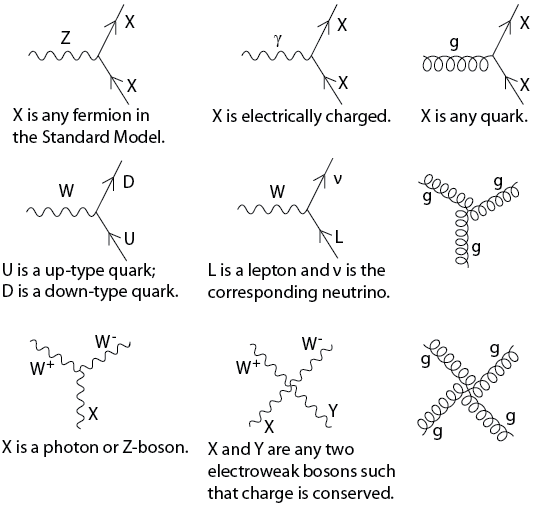
\includegraphics[width=0.7\textwidth]{Figures/Standard_Model_Feynman_Diagram_Vertices.png}
    \caption{
      Fermion and gauge boson vertices of the standard model.
    }
    \label{fig:sm_vertices}
  \end{center}
\end{figure}

The Feynman rule for a vertex includes a coupling constant $g$. These are typically less than 1 in high-energy collisions, meaning diagrams
with additional vertices make smaller contributions to a cross section calculation. Whenever this is the case, we say that
$|\sum_{i}{\mathcal{M}_{i}}|^{2}$ admits a \textit{perturbative expansion}, in which the expression is organized as a sum of terms with increasing powers
of $\alpha \propto g^{2}$, which make successively smaller contributions.
Terms with the lowest powers of $\alpha$ are called leading order (LO) terms, followed by next-to-leading order (NLO), next-to-next-to-leading order (NNLO), etc.
Diagrams with an internal loop contain at least one more vertex than equivalent diagrams without the loop, and therefore \textit{tree-level} diagrams without any internal loops
make the only contributions at LO (when they exist). Each class of interaction has its own characteristic coupling constant:
an $\alpha$ without a subscript usually refers to the fine structure constant characterizing electromagnetic processes, while QCD is characterized by the strong coupling $\alpha_\mathrm{S}$.

In the SM, events with a monophoton signature arise at the LHC (Chap.~\ref{chap:LHCCMS}) primarily from the process $q\bar{q} \to \PZ\Pgamma \to \Pn\Pan\Pgamma$,
where $q$ is any single species of quark, \Pn\ is any single species of neutrino, and the neutrino-antineutrino pair arises from the decay
of a short-lived \PZ\ boson. The leading tree-level diagram for this process is shown in Fig.~\ref{fig:zinvg_diagrams}(a). We typically abbreviate this process by
reference to its final state, \zinvg. The final-state photon can be detected, but the neutrinos only interact with SM particles via the mediation
of \PZ\ and \PW\ bosons, and these interactions are strongly suppressed by the high masses of those particles. Hence, neutrinos almost never interact directly with the LHC's detectors.

\begin{figure}[htb]
  \begin{center}
    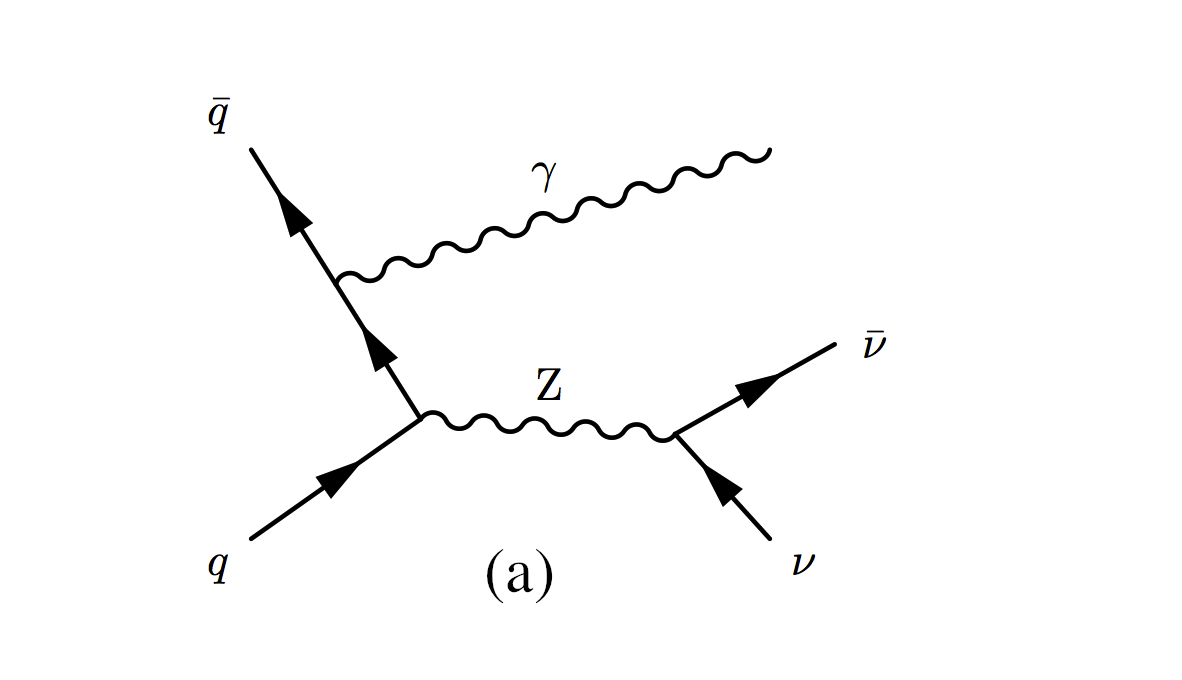
\includegraphics[width=0.49\textwidth]{Figures/zg_isr_v11.pdf}
    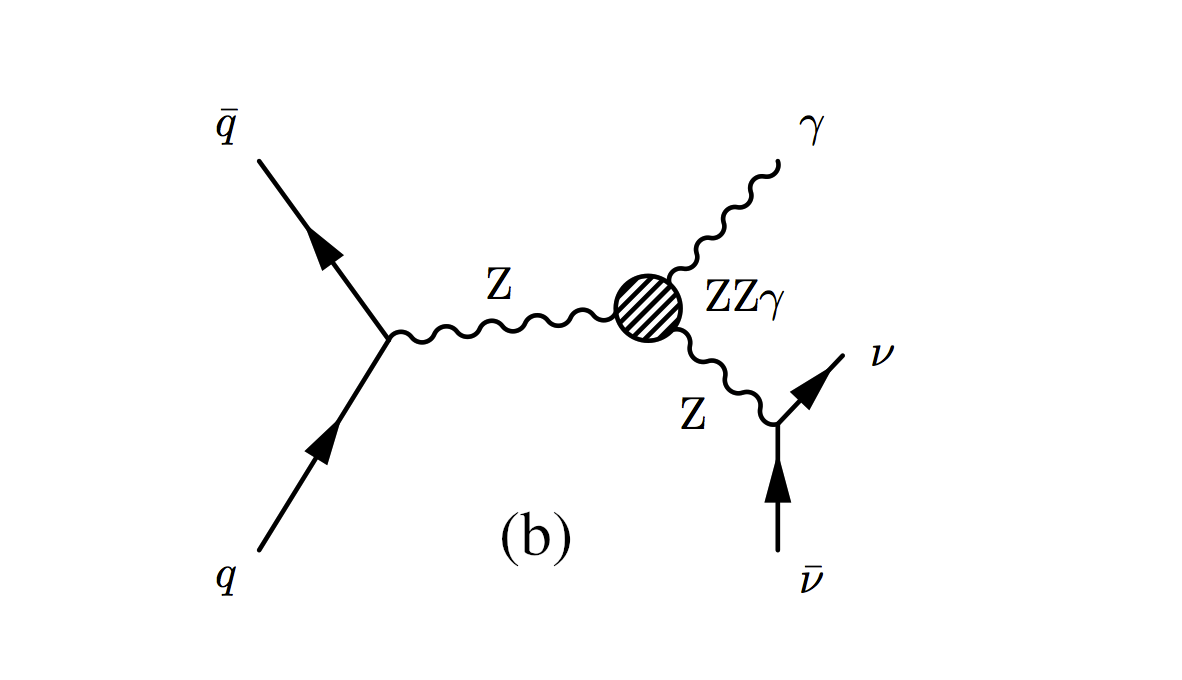
\includegraphics[width=0.49\textwidth]{Figures/zg_zzg_v11.pdf}
    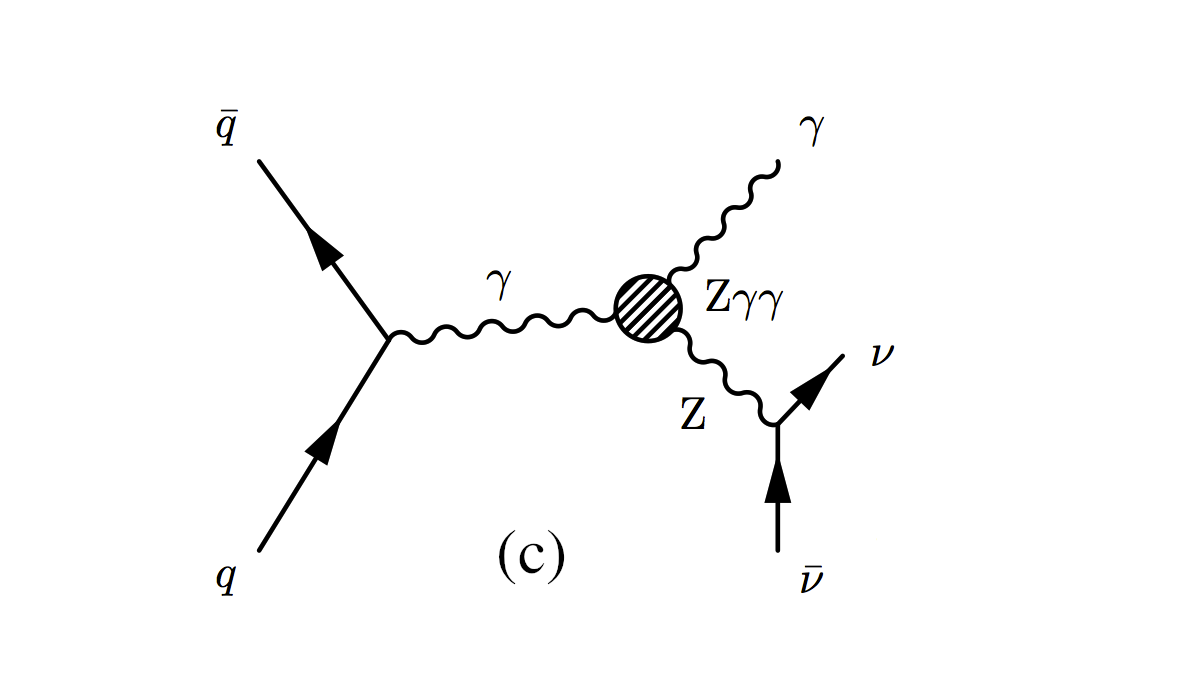
\includegraphics[width=0.49\textwidth]{Figures/zg_zgg_v11.pdf}
    \caption{
      The leading Feynman diagrams for \zinvg\ production arising from \Pp\Pp\ collisions. Diagram (a) is the leading SM contribution.
      Diagrams (b) and (c) show contributions from aTGC vertices.
    }
    \label{fig:zinvg_diagrams}
  \end{center}
\end{figure}

Their existence is instead inferred by their absence.
In a collider experiment, the vectorial momentum transverse to the beam direction, \vecpT, must sum to approximately zero in the reference frame of the
detector. The negative vector sum of \vecpT\ for all detected particles in an event is denoted \vecMET, and its magnitude \MET\ must therefore be close
to zero if all the particles in an event are reliably detected and their momenta are accurately measured. The only high-momentum SM particles that can't
be reliably detected are neutrinos, so a large value of \MET\ can be a sign of neutrino production. An event with a high-\pT\ detected photon, in which
the \vecMET\ has a large magnitude and points in a direction significantly different from that of the photon, is called a monophoton event, and it is
expected that \zinvg\ processes are the main contributors of high-\pT\ monophoton events.

The theoretical SM value for the \zinvg\ cross section has been calculated to NLO in $\alpha$ and $\alpha_\mathrm{S}$~\cite{ref:JHEP04(2015)018, ref:JHEP02(2016)057}.
The \zinvg\ process receives NLO contributions from 1-loop QCD and EWK diagrams, as well as tree-level diagrams with up to one additional radiated \Pgamma, \Pq, or \Pg.
These contributions include diagrams with initial-state $q\bar{q}$, $qg$, and $\bar{q}g$ (with QCD and EWK corrections at NLO), as well as $q\gamma$, $\bar{q}\gamma$ (with EWK corrections
at NLO)~\cite{ref:JHEP02(2016)057}.

The calculation has also been done to NNLO in $\alpha_\mathrm{S}$ alone,
which includes contributions from tree-level diagrams with up to two extra radiated QCD partons (\Pq\ or \Pg), one-loop diagrams with up to one extra
radiated QCD parton, and two-loop corrections. The initial-state QCD parton interactions include those listed among the NLO contributions above,
as well as $gg$~\cite{ref:j.physletb.2014.02.037, ref:JHEP07(2015)085}.

The exact values obtained from any such calculation depend on the specific initial and final states included. These restrictions (\textit{cuts}) on events are
informed by the operating conditions of the experiment one wishes to compare results with.

\subsection{Previous measurements} \label{sec:introduction_znng_previous_measurements}
Experiments at the LEP detector measured the cross section of \zinvg\ arising from $e^{\mathrm{+}}e^{\mathrm{-}}$ collisions for $\sqrt{s}$ up to \textasciitilde200 GeV.
The L3 experiment measured the cross section to be $5.1 \pm 0.3\mathrm{(stat)} \pm 0.1\mathrm{(syst)}$ $pb$ based on 175.6 $pb^{-1}$ of collision data with an average $\sqrt{s} = 188.6$ GeV, compared to an SM
prediction of $4.99 \pm 0.05\mathrm{(stat)}$~\cite{ref:j.physletb.2004.07.002}. Looking at collision data at the same $\sqrt{s}$, but with different cuts,
the OPAL experiment measured the cross section to be $2.52 \pm 0.13\mathrm{(stat)} \pm 0.05\mathrm{(syst)}$ $pb$ based on 177.3 $pb^{-1}$ of data, compared to an SM
prediction of $2.81 \pm 0.02\mathrm{(stat)}$ $pb$~\cite{}. This set of SM predictions were made up to $O(\alpha^2)$, but LO in $\alpha_\mathrm{S}$.

The D0 experiment at the Tevatron made the first observation of \zinvg\ arising from $p\bar{p}$ collisions in 2009. This yielded a cross section measurement of
$32 \pm 9\mathrm{(stat+syst)} \pm 2\mathrm{(lumi)}$ $fb$ for a leading photon \pT\ above 90\unit{GeV}\footnote{The proper units for momentum are $\mathrm{GeV}/c$, but the
factor of $c$ is often omitted for brevity, and this is the convention followed in this thesis.},
compared to an SM prediction of $39 \pm 4\mathrm{(theory)}$ $fb$ computed to NLO in $\alpha_\mathrm{S}$~\cite{ref:PhysRevLett.102.201802}.

Measurements of the cross section at higher values of \pTgamma\ have been performed by experiments examining \Pp\Pp\ collision data at the LHC.
An analysis by the CMS experiment examining 19.6 \fbinv\ of data collected at $\sqrt{s} = 8\unit{TeV}$ found the observed \zinvg\ cross section for $\pTgamma > 145\unit{GeV}$ to be
$52.7 \pm 2.1\mathrm{(stat)} \pm 6.4\mathrm{(syst)} \pm 1.4\mathrm{(lumi)}$ $fb$, compared to an SM prediction of $40.7 \pm 4.9\mathrm{(theory)}$ $fb$ calculated to NLO in $\alpha_\mathrm{S}$, and
a prediction of $50.0^{+2.4}_{-2.2}\mathrm{(theory)}$ calculated to NNLO in $\alpha_\mathrm{S}$~\cite{ref:j.physletb.2016.06.080}. This comparison illustrates the need for NNLO precision at high \pTgamma.

The most precise measurement of the \zinvg\ cross section for \pTgamma\ and \MET\ above 150\unit{GeV} currently comes from an analysis of 36.1 \fbinv\ of \Pp\Pp\ collision data
collected by the ATLAS experiment at $\sqrt{s} = 13\unit{TeV}$, with an observed cross section of $83.7^{+3.6}_{-3.5}\mathrm{(stat)}^{+6.9}_{-6.2}\mathrm{(syst)}^{+1.7}_{-2.0}\mathrm{(lumi)}$ $fb$.
The corresponding SM prediction, computed to NNLO in $\alpha_\mathrm{S}$ using the MATRIX generator~\cite{ref:epjc/s10052-018-5771-7}, is $78.6 \pm 0.4\mathrm{(stat)} \pm 4.1\mathrm{(syst)}$ $fb$~\cite{ref:CERN-EP-2018-220}.
The cross section is shown in discrete ranges (bins) of leading photon \pT\ in Fig.~\ref{fig:znng_xsec_phoET_ATLAS}.

\begin{figure}[hbtp]
  \begin{center}
    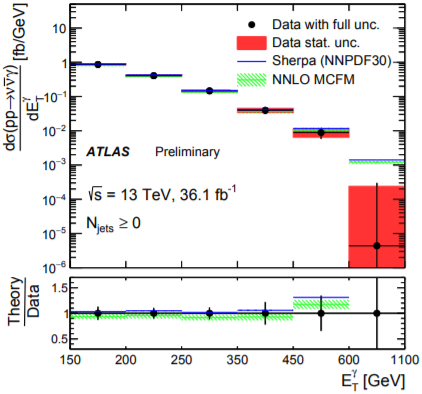
\includegraphics[width=0.4\textwidth]{Figures/znng_xsec_phoET_ATLAS.png}
    \caption{
      Cross section of \zinvg\ production plotted in bins of leading photon \pT\ ($E^{\gamma}_\mathrm{T}$), as shown in~\cite{ref:CERN-EP-2018-220}.
      The blue and green bands show the SM predictions derived from the Sherpa~\cite{ref:1126-6708/2009/02/007} and MCFM~\cite{ref:JHEP07(2011)018} generators, respectively.
    }
    \label{fig:znng_xsec_phoET_ATLAS}
  \end{center}
\end{figure}

None of these analyses report any significant deviation from the SM predictions.

\section{Anomalous triple gauge couplings} \label{sec:introduction_aTGC}
Putative vertices joining three gauge bosons that are not found in the SM are known as aTGCs. For example, there is no fundamental SM vertex
joining a single \Pgamma\ to a pair of \PZ s, or a single \PZ\ to a pair of \Pgamma s. A model
describing the generic phenomenology of these aTGCs is developed in~\cite{ref:Nucl.Phys.0550-3213_87_90685-7, ref:PhysRevD.47.4889, ref:PhysRevD.62.113011}.
For an intermediate state $V = \PZ,\Pgamma$ decaying to a final state \PZ\Pgamma\ pair, this model parametrizes the effective vertex interaction $\PZ V\Pgamma$
by a set of factors $h_{i}^{V}$ ($i$ from 1 to 4). Increasing the values of these parameters significantly increases the cross section
of \zinvg\ processes, by allowing the reaction to proceed via the additional diagrams shown in Fig.~\ref{fig:zinvg_diagrams}(b),(c),
in which the aTGC vertices are covered by opaque circles.

The circle could be thought of as masking a more detailed process taking place underneath. The SM admits processes that are predicted to contribute
to this effective vertex, but all SM contributions to $h_{3,4}^{V}$ have at least one internal loop that could fit within the circle, and
further loops are required for $h_{1,2}^{V}$ contributions~\cite{ref:PhysRevD.47.4889}.
As a consequence, the SM contribution to all eight $h_{i}^{V}$ parameters is quite close to zero.
The observation of a substantial nonzero value for any $h_{i}^{V}$ would be a compelling sign of BSM physics.

The contributions to the \zinvg\ cross section coming from $h_{1,2}^{V}$ are independent of those from $h_{3,4}^{V}$ (for any $V$), and also nearly identical
in magnitude, so without loss of generality we only focus on scenarios for which $h_{3,4}^{V}$ are nonzero. The contributions
from $h_{i}^{\PZ}$ are largely independent of those from $h_{j}^{\Pgamma}$ (for any $i$,$j$), so these are examined separately.
However, the contributions from $h_{3}^{V}$ are substantially correlated with those from $h_{4}^{V}$ (and similarly for $h_{1,2}^{V}$), so we examine
scenarios in which $h_{3,4}^{V}$ take on assorted pairs of values, both of which may be nonzero. The theoretical relationships between these parameters
are explored in~\cite{ref:PhysRevD.47.4889}.

The neutrino decays of \PZ-bosons offer an especially good window on \PZ\PZ\Pgamma\ and \PZ\Pgamma\Pgamma\ aTGCs because the
probability that a \PZ\ will decay into neutrinos is about six times higher than that of a decay into $e^\mathrm{+}e^\mathrm{-}$, or into $\mu^\mathrm{+}\mu^\mathrm{-}$.
Furthermore, the probability of reconstructing a \zinvg\ event in a detector is typically
higher than that of a charged lepton event. As a consequence, aTGC limits derived from neutral \PZ\ decays can be several times
stronger than limits derived from charged \PZ\ decays when analyzing the same \Pp\Pp\ collision data sets (compare e.g.~\cite{ref:PhysRevD.89.092005} and~\cite{ref:JHEP10(2013)164},
based on 7\unit{TeV} LHC data; also Fig.~\ref{fig:lhc_8tev_atgc_1dlimits}, based on 8\unit{TeV} data).
The decays of \PZ\ into $q\bar{q}$ (and thence to hadrons) are difficult to distinguish in practice from hadronic \PW\ decays~\cite{ref:RevModPhys.89.035008}.

\subsection{Previous searches} \label{sec:introduction_aTGC_previous_searches}
The LEP collider established constraints on each of the eight the parameters $h_{i}^{V}$ in the context of the process $e^{\mathrm{+}}e^{\mathrm{-}} \to \PZ\Pgamma$.
In a statistical combination of searches perfomed by the DELPHI, L3, and OPAL experiments, examining 3 \fbinv\ of $e^{\mathrm{+}}e^{\mathrm{-}}$ collision data
for $\sqrt{s}$ ranging from 130 GeV to 209 GeV, the 95\% CL intervals of seven of the parameters contain 0, with total ranges between 0.05 and 0.10 for $h_{i}^{\Pgamma}$
and between 0.14 and 0.25 for $h_{i}^{\PZ}$; the 95\% CL interval for the remaining factor $h_{4}^{\gamma}$ spans 0.01 to 0.05~\cite{ref:j.physrep.2013.07.004}.

The LEP combined analysis assumed that all but one of the eight parameters were fixed to the SM expectation of 0 (i.e. these are 1D limits).
It was also the last major effort to obtain limits on $h_{1,2}^{V}$ independently of $h_{3,4}^{V}$,
as subsequent searches have taken the present approach of focusing on $h_{3,4}^{V}$ alone, for the reasons listed above.
Uniquely among the LEP experiments, the L3 Collaboration also placed limits on correlated pairs of parameters (2D limits), shown in Fig.~\ref{fig:L3_atgc_contours}~\cite{ref:j.physletb.2004.07.002}.

\begin{figure}[hbtp]
  \begin{center}
    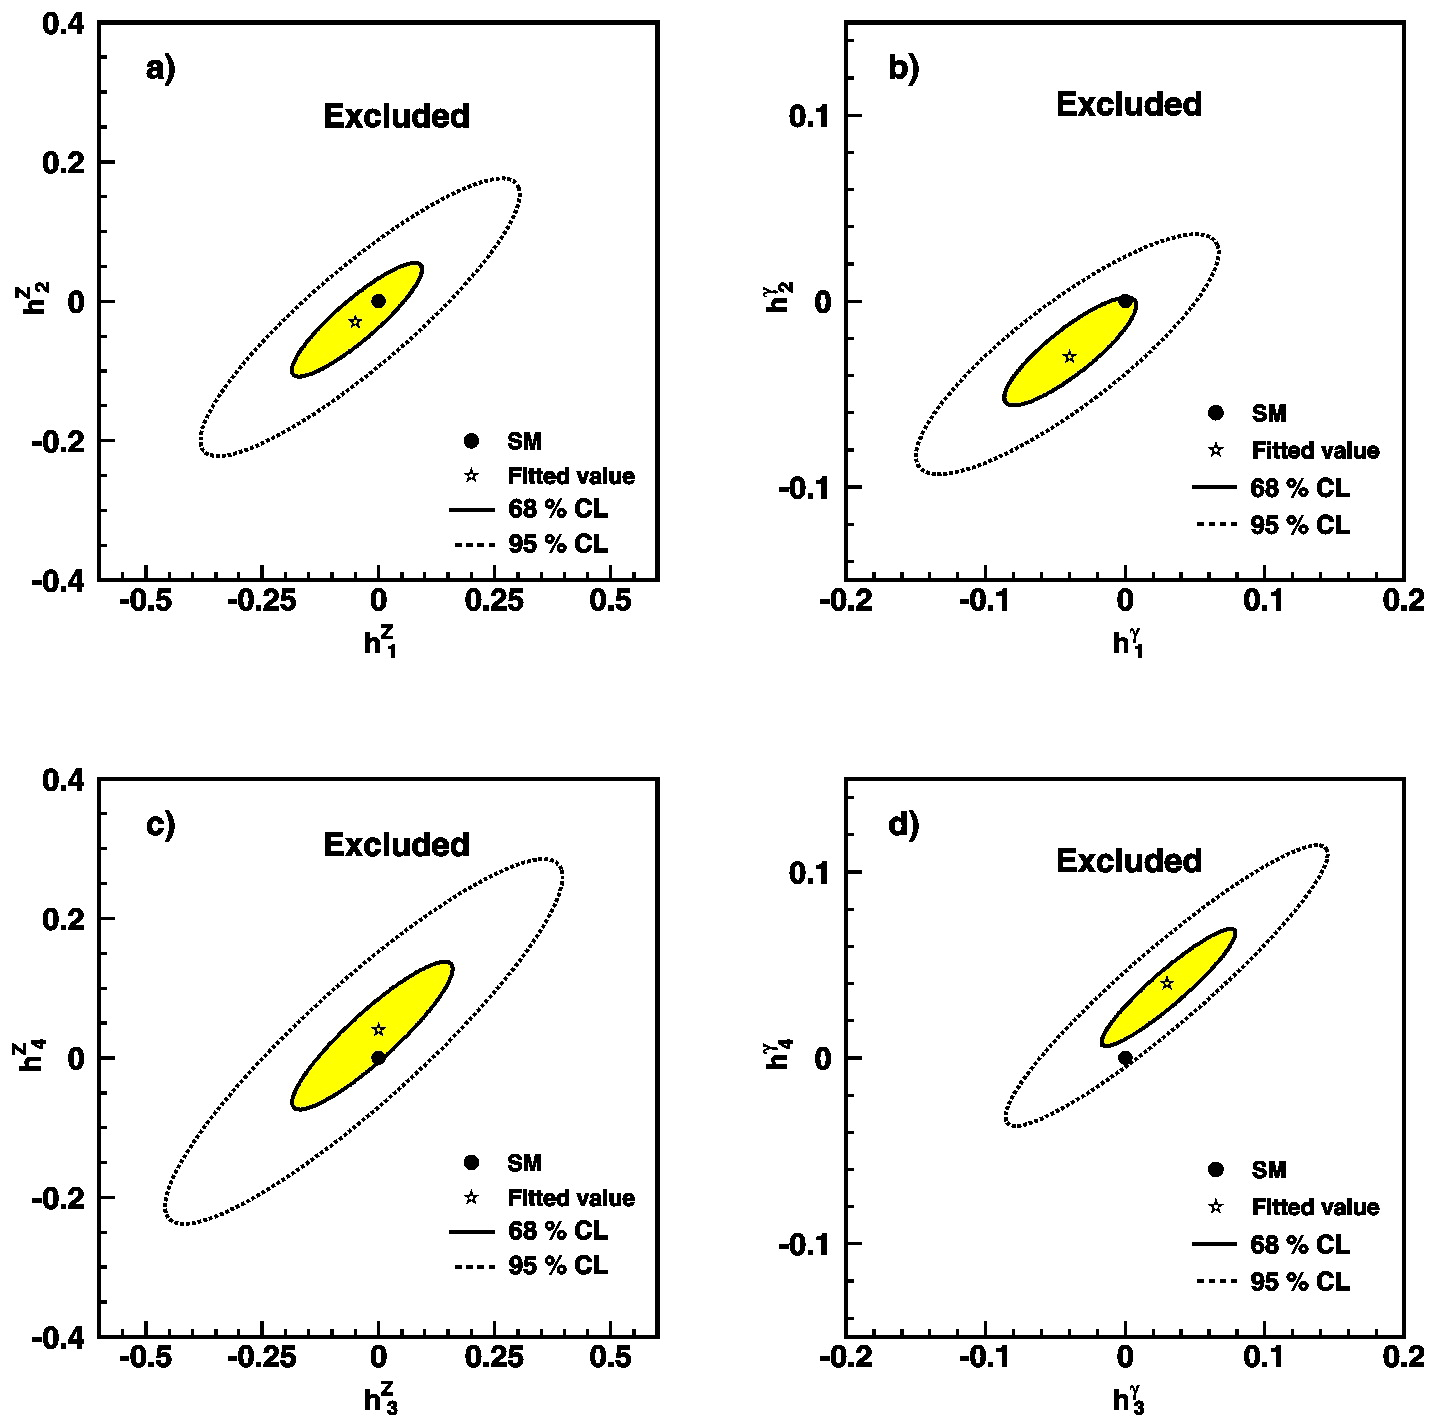
\includegraphics[width=0.8\textwidth]{Figures/L3_atgc_contours.jpg}
    \caption{
      $h_{i}^{V}$ exclusion contours from the L3 experiment at the LEP collider, as shown in~\cite{ref:j.physletb.2004.07.002}.
    }
    \label{fig:L3_atgc_contours}
  \end{center}
\end{figure}

Experiments at the Tevatron collider improved these limits in analyses of $p\bar{p}$ collision data at $\sqrt{s} = 1.96\unit{TeV}$.
The Tevatron analyses incorporated a form factor $1 / (1 + \hat{s}/\Lambda^{2})^{n}$, by which a constant term $h_{0i}^{V}$ is
multiplied to obtain $h_{i}^{V}$.
The form factor is essentially arbitrary; $n$ is set equal to $i$ and $\Lambda$ (not to be confused with the EFT suppression scale, below)
is set to 1.5\unit{TeV} by convention. This form factor was introduced in the common reference~\cite{ref:PhysRevD.47.4889} but was not used in LEP~\cite{ref:j.physrep.2013.07.004}
or most subsequent LHC analyses, which treat the $h_{i}^{V}$ parameters as constants independent of $\hat{s}$.

The CDF experiment combined analyses of \zinvg\ processes, using 4.9 \fbinv\ of data, and processes where the \PZ\ decays to
$l^\mathrm{+}l^\mathrm{-}$ ($e^\mathrm{+}e^\mathrm{-}$ or $\mu^\mathrm{+}\mu^\mathrm{-}$), using 5.1 \fbinv\ of data.
They set 95\%\ Bayesian credibility intervals constraining $|h_{3}^{V}| < 0.022$ and $|h_{4}^{V}| < 0.0009$ (1D limits)~\cite{ref:PhysRevLett.107.051802}.
The D0 experiment similarly combined a 3.6 \fbinv\ \zinvg\ analysis with a 7.2
\fbinv\ $Z(l^\mathrm{+}l^\mathrm{-})\gamma$ analysis to set 95\%\ CL limits constraining
$|h_{03}^{V}| < 0.027$ and $|h_{04}^{V}| < 0.0014$ (1D limits)~\cite{ref:PhysRevD.85.052001}. Correlated 2D limits were also
computed and are shown in Fig.~\ref{fig:d0_aTGC}.

\begin{figure}[hbtp]
  \begin{center}
    \includegraphics[width=0.45\textwidth]{Figures/d0_ZZg.png}
    \includegraphics[width=0.45\textwidth]{Figures/d0_Zgg.png}
    \caption{
      $h_{0i}^{V}$ exclusion contours from the D0 experiment at the Tevatron collider, from~\cite{ref:PhysRevD.85.052001}.
    }
    \label{fig:d0_aTGC}
  \end{center}
\end{figure}

Experiments at the LHC made further improvements via the analysis of \Pp\Pp\ collision data at progressively higher $\sqrt{s}$.
A summary of 1D limits on $h_{i}^{V}$ from both the ATLAS and CMS experiments obtained from analyses of \textasciitilde20 \fbinv\ of $\sqrt{s} = 8\unit{TeV}$ data
is shown in Fig.~\ref{fig:lhc_8tev_atgc_1dlimits}. ATLAS limits show the results of combined \zinvg\ and $Z(l^\mathrm{+}l^\mathrm{-})\gamma$
analyses, both with and without a form factor on $h_{i}^{V}$. CMS limits show separate \zinvg\ results, along with $Z(l^\mathrm{+}l^\mathrm{-})\gamma$
results, both without a form factor~\cite{ref:RevModPhys.89.035008}. These comparisons make clear that \zinvg\ is by far
the more sensitive channel for setting aTGC limits.

\begin{figure}[hbtp]
  \begin{center}
    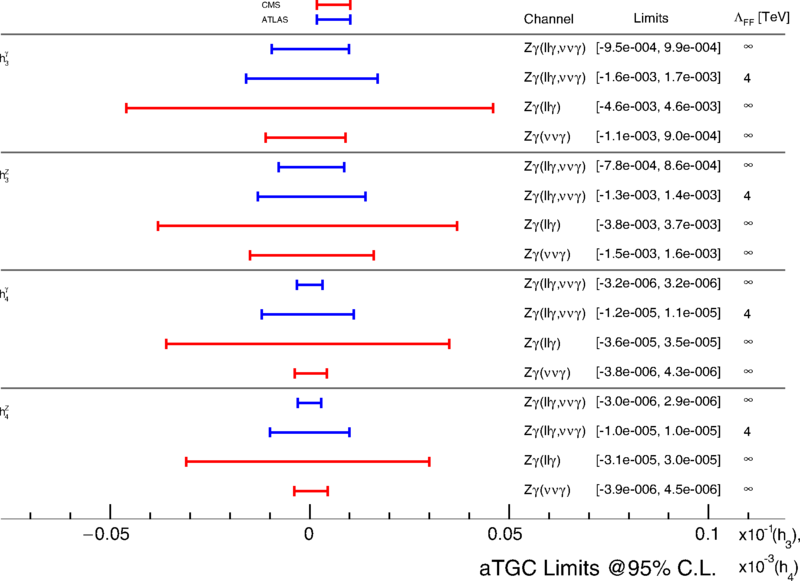
\includegraphics[width=\textwidth]{Figures/lhc_8tev_atgc_1dlimits.png}
    \caption{
      1D $h_{i}^{V}$ exclusion limits from the ATLAS and CMS experiments at the LHC based on 20 \fbinv\ of $\sqrt{s} = 8\unit{TeV}$
      \Pp\Pp\ collision data, from~\cite{ref:RevModPhys.89.035008}.
      $Z\gamma(ll\gamma)$ indicates a combination of $Z(e^\mathrm{+}e^\mathrm{-})\gamma$ and $Z(\mu^\mathrm{+}\mu^\mathrm{-})\gamma$
      analyses; $Z\gamma(ll\gamma,\nu\nu\gamma)$ indicates a combination of these with \zinvg. The mass $\Lambda_{FF}$
      is the form factor scale; $\infty$ means no form factor was used.
    }
    \label{fig:lhc_8tev_atgc_1dlimits}
  \end{center}
\end{figure}

The most sensitive published limits on $h_{3,4}^{Z,\gamma}$ are currently derived from 36.1 \fbinv\ of 13\unit{TeV} \Pp\Pp\ collision
data collected by the ATLAS detector at the LHC, analyzed exclusively in the monophoton channel, with no form factor~\cite{ref:CERN-EP-2018-220}.
These are summarized in Figs.~\ref{fig:atlas_atgc_13tev_1dlimits},~\ref{fig:atlas_atgc_13tev_2dlimits}.

\begin{figure}[hbtp]
  \begin{center}
    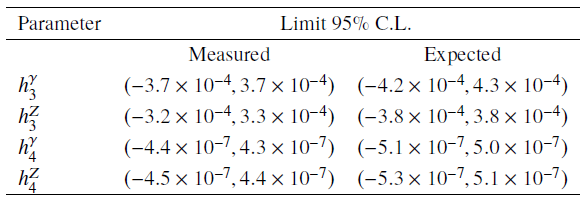
\includegraphics[width=0.8\textwidth]{Figures/atlas_atgc_13tev_1dlimits.png}
    \caption{
      1D $h_{i}^{V}$ exclusion limits from the ATLAS experiment at the LHC based on 36.1 \fbinv\ of $\sqrt{s} = 13\unit{TeV}$
      \Pp\Pp\ collision data, analyzed in the monophoton channel, as shown in~\cite{ref:CERN-EP-2018-220}.
    }
    \label{fig:atlas_atgc_13tev_1dlimits}
  \end{center}
\end{figure}

\begin{figure}[hbtp]
  \begin{center}
    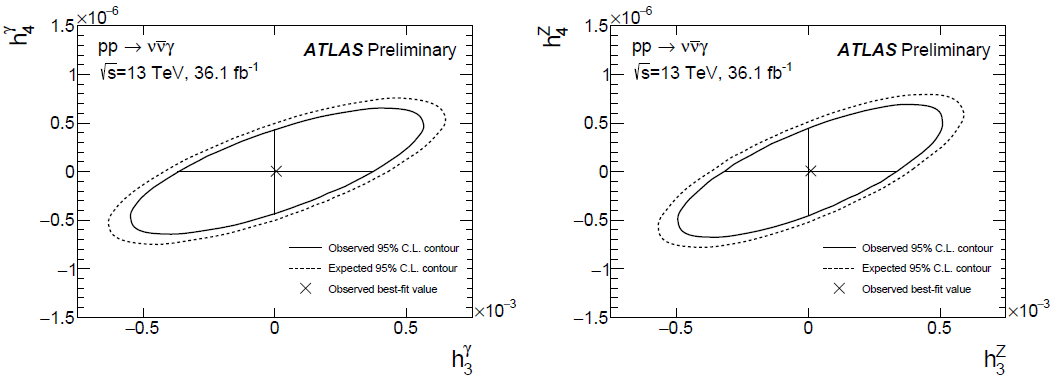
\includegraphics[width=\textwidth]{Figures/atlas_atgc_13tev_2dlimits.png}
    \caption{
      2D $h_{i}^{V}$ exclusion contours from the ATLAS experiment at the LHC based on 36.1 \fbinv\ of $\sqrt{s} = 13\unit{TeV}$
      \Pp\Pp\ collision data, analyzed in the monophoton channel, as shown in~\cite{ref:CERN-EP-2018-220}.
    }
    \label{fig:atlas_atgc_13tev_2dlimits}
  \end{center}
\end{figure}

None of these analyses report any significant evidence of BSM physics.

\section{Dark matter EFT and simplified models} \label{sec:introduction_dm}
The standard theory of gravitation, Einstein's
general theory of relativity (GR), has passed experimental tests over scales ranging from the orbits of satellites~\cite{ref:lrr-2003-1} to the entire observable universe~\cite{ref:planck2018_cosparams},
matching observations more closely than Newton's theory of gravitation, to which it converges in the weak-field limit~\cite{ref:WaldGR}.
It predicts the existence of gravitional waves, directly detected for the first time in 2015~\cite{ref:PhysRevLett.116.061102}, and these have been used to test the theory in the strong-field regime~\cite{ref:PhysRevLett.116.221101}.

Despite its many triumphs, GR fails---under the assumption that SM particles and their known interactions are the only sort that exist---to describe the orbits of stars in nearly every galaxy~\cite{ref:nature25767},
the average weak distortion of light by galaxies~\cite{ref:weaklensing}, the strong distortion of light by galaxy clusters~\cite{ref:mnras/stw3385}, the orbits of galaxies in galaxy clusters~\cite{ref:annurev-astro-081710-102514},
the formation of large-scale filamentary structures~\cite{ref:nature03597}, or the distribution of ripples in the cosmic microwave background (CMB) arising from big bang nucleosynthesis~\cite{ref:planck2018_cosparams}.
Each of these phenomena could be explained by the existence of an abundance of massive matter with no discernible interactions of any sort, other than gravitation.
This extends to interactions with visible light, giving rise to the name ``dark matter.''

These difficulties could also indicate the need to modify the theory of gravity.
However, the nature of the Bullet cluster, a galaxy cluster with a center of mass displaced from its visible mass center, is challenging to explain in a theory of gravity without DM that can also explain all of
the preceding observations. In contrast, it has a straightfoward explanation if GR+DM is true: the displaced mass is DM~\cite{ref:508162}. Furthermore, if a modified theory of gravity
results in the apparent gravitational effect of DM on galactic scales, then the existence of a galaxy without any apparent DM, as observed in~\cite{ref:nature25767}, is
also challenging to explain. It's conceivable that a random collection of stars could agglomerate into a galaxy without the assistance of DM, or else become separated from their
DM component (as with the Bullet cluster), but the fundamental laws of gravitation should not fail in just one galaxy.

No SM particle is predicted to exhibit the behavior of DM, and this has spurred the development
of BSM theories describing new particles that could account for it~\cite{ref:s41550-017-0059, ref:j.physrep.2004.08.031, ref:annurev.nucl.54.070103.181244, ref:S1062798717000783}.
The great diversity of theories motivates general models that can potentially constrain a wide variety of specific theories simultaneously.
If DM is particulate in nature, it apparently has a substantial mass, interacts very weakly with SM particles, and is stable on cosmological timescales~\cite{}.
The models we consider here include a BSM particle satisfying each of these criteria.
All the massive, stable particles in the SM are fermionic, and these models similarly describe a fermionic DM candidate. Otherwise, the new physics
content of these models is kept to a minimum, as sufficiently large deviations from SM predictions would presumably have been detected by now.

One model we examine describes a direct coupling between DM and the neutral EWK vector bosons \PZ\ and \Pgamma~\cite{ref:PhysRevD.89.056011}. The model does not fully specify
the nature of the proposed particle and its SM interactions, but rather only predicts the most dominant potential signature of new physics,
by adding a handful of new operator terms to the SM Lagrangian. Any operator has a \textit{mass dimension}, denoted in powers of GeV. The SM Lagrangian has
a mass dimension of 4, and any operator term added to it has to have this same mass dimension for the expression to be coherent.
Additional particle interactions in an operator term tend to raise the mass dimension. If an operator describes an especially intricate interaction,
the overall term must be multiplied by an extra factor of $(\frac{1}{\Lambda})^{n}$ to maintain an overall mass dimension of 4, where $\Lambda$ is some mass
scale in GeV and $n$ is a positive number.

Operator terms with nonzero powers of $\frac{1}{\Lambda}$ tend to have their interactions suppressed for interaction energies much
smaller than $\Lambda$, and so $\Lambda$ is called the \textit{suppression scale}. The effects of more complicated terms, multiplied by higher powers of $\frac{1}{\Lambda}$,
are expected to become apparent at higher interaction energy scales, so a model that only incorporates simpler terms is expected to
lose predictive validity as the interaction energy approaches $\Lambda$~\cite{ref:j.aop.2013.04.016}. A model that only adds a restricted set of terms,
with predictive validity only up to energies below $\Lambda$, is called an EFT.

The DM-EWK EFT described in~\cite{ref:PhysRevD.89.056011} adds four dimension-7 interaction terms to the SM Lagrangian, which therefore carry factors of $\frac{1}{\Lambda}$
raised to the third power. The mass $m_\mathrm{DM}$ of the new DM particle is a free parameter of the model, along with two constants $k_1$ and $k_2$ controlling
the relative strengths of the DM-\PZ\ and DM-\Pgamma\ couplings.
Fig.~\ref{fig:dm_diagrams} illustrates the dominant contribution of this interaction to monophoton yields. Since the DM
particle only interacts with the \PZ\ and \Pgamma, and this interaction is suppressed by $(\frac{1}{\Lambda})^{3}$, the outgoing DM is not expected to interact
with any detector elements.

\begin{figure}[hbtp]
  \begin{center}
    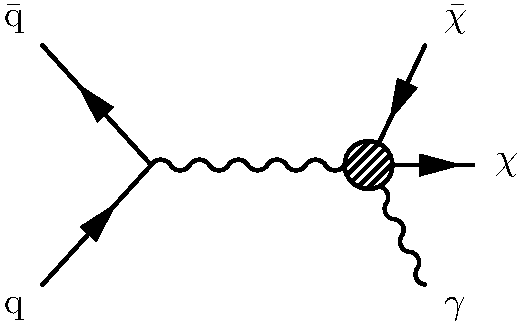
\includegraphics[width=0.42\textwidth]{Figures/dmewk.pdf}
    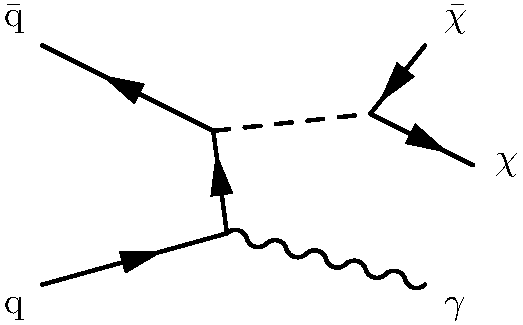
\includegraphics[width=0.42\textwidth]{Figures/dm.pdf}
    \caption{
      Leading order Feynman diagrams for monophoton processes in a DM-EWK EFT (left) and in DM simplified models (right).
      The intermediate boson in the EFT diagram can be a \PZ\ or \Pgamma. The dotted line in the DM simplified model diagram
      stands for the DM-quark mediator.
    }
    \label{fig:dm_diagrams}
  \end{center}
\end{figure}

Since the DM pair emerges directly from an EWK boson, this EFT is limited in the dynamics it can describe. In contrast, so-called \textit{simplified models} of DM add
a new mediating boson between the DM and SM fermions~\cite{ref:1507.00966}, which more typically characterizes the fermion interactions that we know
from the SM. These models are still ``simplified'' in that they fall short of a complete theory of particle physics valid in all contexts---for example,
the DM lacks a coupling to the \PH, but still has mass. Nevertheless, some kind of DM--mediator--SM interaction is a generic feature of many new physics models,
and so limits on the strength of this interaction potentially constrain a broad class of more specific models.

We examine models in which the mediator has either exclusively vector or exclusively axial-vector couplings to DM and also to SM quarks, independently
of quark flavor. The free parameters of this model include
the DM mass $m_\mathrm{DM}$, the mediator mass $M_\mathrm{med}$, the DM-mediator coupling $g_\mathrm{DM}$ and the DM-quark coupling $g_\mathrm{q}$.
The leading Feynman diagrams for monophoton production are shown in Fig.~\ref{fig:dm_diagrams}. The mediators are typically chosen to be quite massive,
which suppresses the likelihood of DM-quark interactions, and the mediator does not have any direct couplings to leptons or bosons,
so the DM is not expected to interact with detector elements as it escapes.

\subsection{Previous searches} \label{sec:introduction_dm_previous_searches}
In the limit that $M_\mathrm{med}$ is much larger than the $q\bar{q}$ interaction energy, DM simplified models converge to an EFT describing a direct contact
interaction between DM and quarks, with a suppression scale $M_\mathrm{*} = M_\mathrm{med}/\sqrt{g_\mathrm{q}g_\mathrm{DM}}$~\cite{ref:1603.04156}.
Such DM-quark EFT models were the subject of monophoton searches~\cite{ref:j.physletb.2016.01.057, ref:PhysRevD.91.012008} prior to the adoption of
DM simplified models by the ATLAS-CMS Dark Matter Forum in 2015~\cite{ref:1507.00966}.
As the interaction energy increases, the EFT description breaks down for the reasons described above, and DM simplified models
offer a replacement that retains predictive validity (at the cost of some degree of generality).
In contrast, the dimension-7 DM-EWK EFT considered here is not the large-$M_\mathrm{med}$ limit of a DM simplified model~\cite{ref:1507.00966} and represents a truly distinct
process topology.

Both the DM simplified models and the DM-EWK EFT were developed after LHC data taking began, with comparisons to LHC data in mind~\cite{ref:1507.00966, ref:PhysRevD.89.056011}.
Thus, the history of examination of these models begins with analyses of data collected by the ATLAS and CMS experiments at the LHC.
In general, limits on BSM models set by LHC experiments become stronger at higher energies and with larger data sets.
The remainder of this section describes the most stringent experimental limits set by the ATLAS and CMS experiments, each based on analyses of 13\unit{TeV} \Pp\Pp\ collision data
collected in 2016.

New physics introduced by DM simplified models is expected to contribute to a variety of other signatures in addition to the monophoton signature. Figure~\ref{fig:dmsimp_ichep2018} compares
analyses in three different ``mono-X'' channels based on data collected by the CMS detector, including the most recent monophoton results described herein. Each of the three
searches examine similar final state characteristics; they are primarily distinguished by the type of particle(s) emerging against the \vecMET, listed in the caption.
The limits on DM simplified model parameters set by the monophoton search are generally more stringent than those set by mono-$Z$ search, but less stringent
than those set by the mono-$j/V$ search. The concordance of results from each of these three independent analyses reinforces the degree of confidence with which model
parameters are excluded, and in the event of a new physics discovery in one channel, the nature of the discovery will be further illuminated by searching for a corroborating
signature in other channels.

\begin{figure}[hbtb]
  \begin{center}
    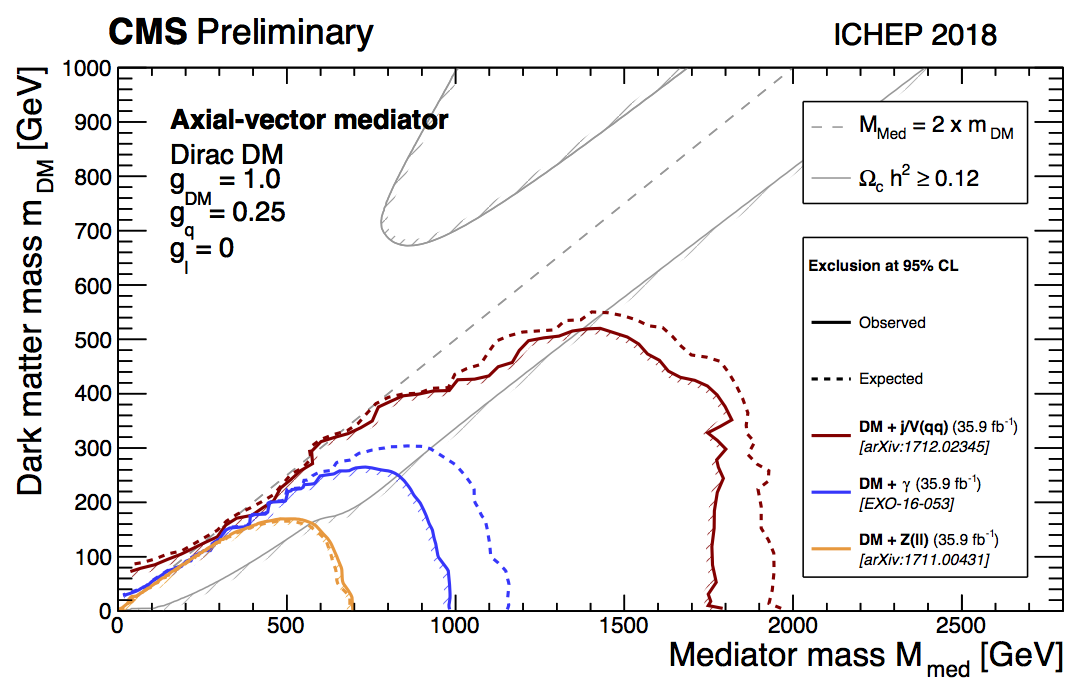
\includegraphics[width=0.49\textwidth]{Figures/dmsimp_ichep2018_av.png}
    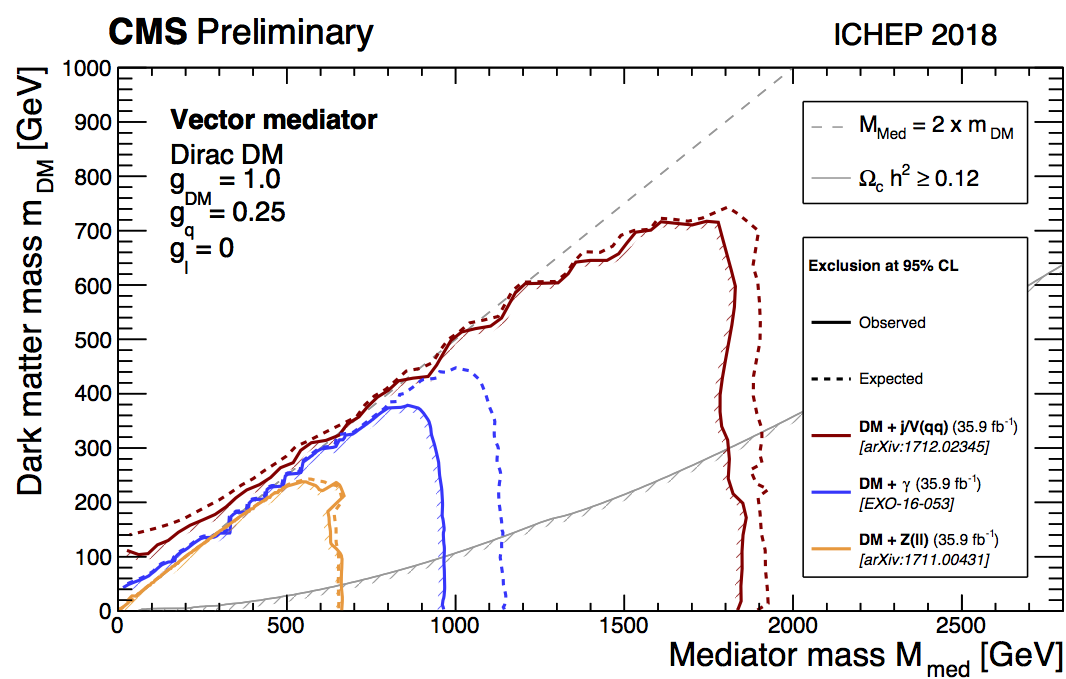
\includegraphics[width=0.49\textwidth]{Figures/dmsimp_ichep2018_v.png}
    \caption{Summary plots of limits on DM simplified model parameters, shown in~\cite{ref:dmsummaryplots_ichep2018}. Simplified models are excluded at 95\% CL or above
    for parameter values under the contours.
    Results based on three different final states are shown: mono-$Z(ll)$~\cite{ref:epjc/s10052-018-5740-1} in yellow, mono-$j/V(qq)$~\cite{ref:PhysRevD.97.092005} in red, and monophoton~\cite{ref:1810.00196} in blue,
    the latter corresponding to the new results presented in this thesis. The $\Omega_\mathrm{c}^{2}$ curves correspond to constraints on the cosmological DM abundance set by Planck satellite measurements~\cite{ref:planck2018_cosparams}.}
    \label{fig:dmsimp_ichep2018}
  \end{center}
\end{figure}

Prior to the analysis presented in this thesis, the last published results from CMS in the monophoton final state examined 12.9 \fbinv\ of data collected in the first half
of 2016~\cite{ref:JHEP10(2017)073}. Simplified models were excluded at 95\% CL for $M_\mathrm{med}$ up to 700 GeV at small values of $m_\mathrm{DM}$, in both the vector
and axial-vector cases. Values of $\Lambda$ for the DM-EWK EFT up to 600 GeV were also excluded at 95\% CL, assuming $k_{1} = k_{2} = 1$\footnote{Defining $k = \sqrt{k_{1}^{2} + k_{2}^{2}}$
and $\theta_{k} = \arctan{\frac{k_{2}}{k_{1}}}$, the choice $k_{1} = k_{2} = 1$ corresponds to the choice $k = \sqrt{2}$ and $\theta_{k} = \pi/4$. Fixing $\theta_{k} = \pi/4$,
the limits on $\Lambda / k^{1/3}$ for arbitrary $k$ are equal to the $k = \sqrt{2}$ limits on $\Lambda$ multiplied by $2^{-1/6}$.}.

The most stringent monophoton results to date are set by an analysis of 36.1 \fbinv\ of data collected by the ATLAS detector~\cite{ref:epjc/s10052-017-4965-8}.
Simplified models were excluded at 95\% CL for $M_\mathrm{med}$ up to 1200 GeV at small values of $m_\mathrm{DM}$, in both the vector and axial-vector cases, as shown in Fig.~\ref{fig:dmsimp_atlas}.
Values of $\Lambda$ for the DM-EWK EFT up to 790 GeV, assuming $k_{1} = k_{2} = 1$, were also excluded at 95\% CL, as shown in Fig.~\ref{fig:dmeft_atlas}.

Assuming DM simplified models describe the dominant mode of interaction between DM and SM particles, the scattering cross section of low-energy (nonrelativistic) DM off nucleons (protons and neutrons)
is uniquely determined~\cite{ref:1603.04156}. This allows DM simplified model limits to be compared directly with limits set by \textit{direct detection} (DD) experiments, which search for freely-floating
ambient DM by looking for signatures of DM scattering off of target nuclei.
The most recent ATLAS results are plotted against a variety of DD limits in Fig.~\ref{fig:dmsimp_dd_atlas}. An axial-vector/vector mediator corresponds to a DM-nucleus cross section
that does/does not depend on the spin of the nucleus, respectively known as the spin-dependent/spin-independent (SD/SI) cross section.

\begin{figure}[hbtb]
  \begin{center}
    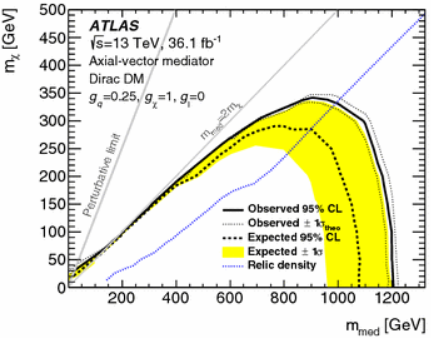
\includegraphics[width=0.49\textwidth]{Figures/dmsimp_atlas_av.png}
    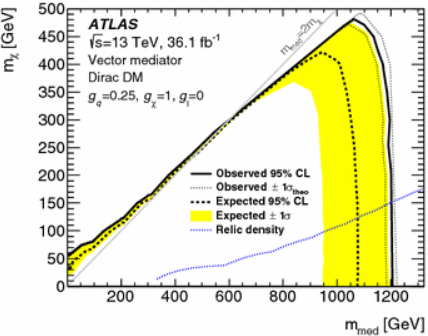
\includegraphics[width=0.49\textwidth]{Figures/dmsimp_atlas_v.png}
    \caption{Limits on DM simplified model parameters set by the ATLAS experiment, as shown in~\cite{ref:epjc/s10052-017-4965-8}. Simplified models are excluded at 95\% CL or above
    for parameter values under the contours. The relic density curves correspond to constraints on the cosmological DM abundance set by Planck satellite measurements~\cite{ref:planck2018_cosparams}.
    }
    \label{fig:dmsimp_atlas}
  \end{center}
\end{figure}

\begin{figure}[hbtb]
  \begin{center}
    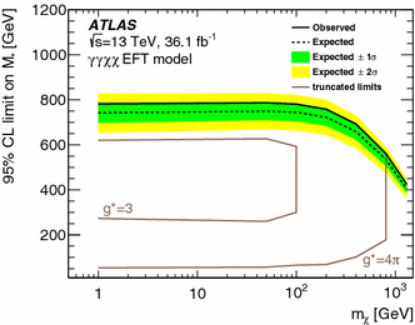
\includegraphics[width=0.49\textwidth]{Figures/dmeft_atlas.png}
    \caption{Limits on the DM-EWK EFT set by the ATLAS experiment, as shown in~\cite{ref:epjc/s10052-017-4965-8}. The DM-EWK EFT is excluded at 95\% CL or above for
    values of $\Lambda$ under the contour.
    }
    \label{fig:dmeft_atlas}
  \end{center}
\end{figure}

\begin{figure}[hbtb]
  \begin{center}
    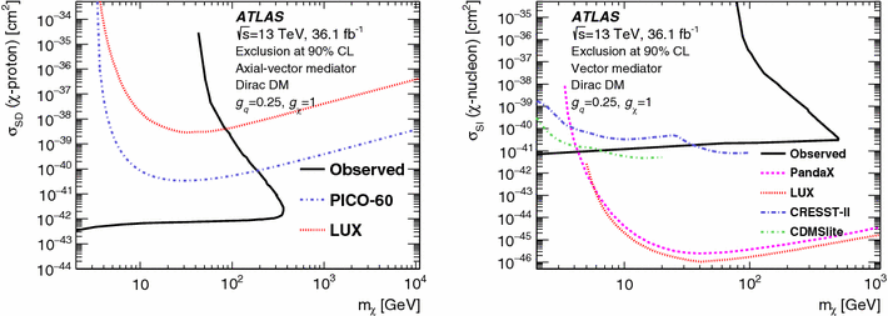
\includegraphics[width=0.98\textwidth]{Figures/dmsimp_dd_atlas.png}
    \caption{Limits on low-energy DM-nucleon scattering cross sections set by the ATLAS experiment, as shown in~\cite{ref:epjc/s10052-017-4965-8}. The ATLAS
    limits are compared against limits on the SD cross section from PICO-60~\cite{ref:PICO60-ATLAS} and LUX~\cite{ref:LUX-SD-ATLAS} (left)
    and limits on the SI cross section from PandaX-II~\cite{ref:PANDAX-II-ATLAS}, LUX~\cite{ref:LUX-SI-ATLAS}, CRESST-II~\cite{ref:CRESST-II-ATLAS}, and CDMSlite~\cite{ref:SuperCDMS-ATLAS} (right).
    Scattering cross sections are excluded at 90\% CL or more above the contours.
    }
    \label{fig:dmsimp_dd_atlas}
  \end{center}
\end{figure}

All of the preceding limits were derived for $g_\mathrm{DM} = 1$ and $g_\mathrm{q} = 0.25$, which matches the couplings used for the results obtained herein.
By convention, this is the most commonly investigated set of values for these couplings, but studies have been done using alternative values, some of which
include a small nonzero coupling between the new mediator and charged leptons (e.g.~\cite{ref:epjc/s10052-017-4965-8}).

None of these analyses report any significant evidence of BSM physics.

\section{ADD gravitons} \label{sec:introduction_ADD}
We finally examine a model of gravitation in extra dimensions originally proposed by Arkani-Hamed, Dimoupolos, and Dvali (ADD)~\cite{ref:S0370-2693(98)00466-3}.
Gravity typically affects SM particles much, much less than the other fundamental interactions. The weakness of gravity
is often expressed in terms of a fundmental mass scale $M_\mathrm{Pl}$ (\textasciitilde$10^{19}$ GeV), which is
many orders of magnitude larger than the masses of the EWK bosons (\textasciitilde$10^{2}$ GeV). Particle-level gravitational interactions
are correspondingly sharply suppressed. The proposed boson of gravitation, the graviton, has yet to be detected and is not part of the SM.
The mystery of why $M_\mathrm{Pl}$ is so much larger than the EWK mass scale has been called the ``Hierarchy problem,'' and the desire for a
more elegant formulation has been a productive stimulus for BSM theories~\cite{ref:S0370-2693(98)00466-3, ref:0264-9381/32/3/033001}.

Everyday experience indicates that there are 3 dimensions of space and 1 dimension of time, and the SM assumes this to be true.
The ADD model begins with the observation that, if there are $n$ extra spatial dimensions beyond the usual 3,
we might not be able to directly perceive them if all the SM particles are confined by some as-yet-unspecified
mechanism to a 3+1-dimensional subspace (the ``brane'') of the full $n$+3+1-dimensional spacetime (the ``bulk'')\footnote{The case $n=0$ corresponds
to ordinary GR.}.
In contrast, gravitons in this model are able to propagate freely throughout the bulk.

Gravitation in the bulk is characterized by a mass scale $M_\mathrm{D}$ distinct from the mass scale $M_\mathrm{Pl}$ that
characterizes gravitation as perceived by particles confined to the brane. If the extra dimensions are not extended infinitely like the
dimensions of common experience, but rather ``compactified'' into a finite volume of characteristic radius $R$, then for a sufficiently mild
energy density in the vicinity of the brane, $M_\mathrm{Pl}^{2} \approx M_\mathrm{D}^{n+2} R^{n}$~\cite{ref:S0370-2693(98)00466-3, ref:S0550-3213(99)00044-9}.
For a modest number of extra dimensions (e.g. $3 \leq n \leq 6$), the observed large value of $M_\mathrm{Pl}$ could then really
be a consequence of a large value for $R$, while the fundamental gravitational scale $M_\mathrm{D}$ could be closer to or even
the same as the EWK scale. In light of this possibility, ADD model predictions are typically examined for values of $M_\mathrm{D}$ in the vicinity of 1\unit{TeV}.

The cross sections for a variety of graviton production scenarios are calculated in ref.~\cite{ref:S0550-3213(99)00044-9}, using a low-energy EFT
approximation of GR in which $M_\mathrm{D}$ serves as the suppression scale. At higher energies the specific details of the geometry of the extra dimensions,
and phenomena uniquely predicted by a full quantum theory of gravitation, would start to become apparent. These are both unknown, and the EFT correspondingly
does not make predictions on the outcome of scattering events with energies above $M_\mathrm{D}$.

The ratio $M_\mathrm{Pl} / M_\mathrm{D}$ essentially expresses the wide range of kinematic possibilities that open up for gravitons with the addition
of extra dimensions. After summing over all of these possibilities, the resulting
cross section is high enough for graviton production to be probed with existing collider experiments.
Gravitons couple to every SM particle, although the coupling is still sufficiently weak that an emitted graviton will generally not interact with a detector element.
This results in a monophoton signature if it is emitted opposite a photon, as illustrated in Fig.~\ref{fig:add_diagram}.

\begin{figure}[hbtp]
  \begin{center}
    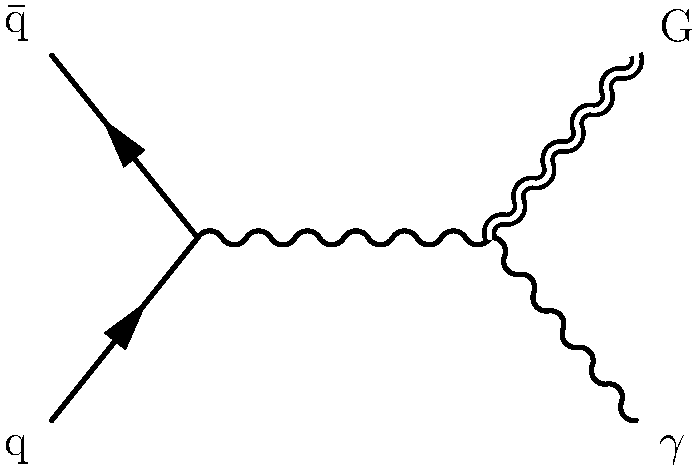
\includegraphics[width=0.42\textwidth]{Figures/add.pdf}
    \caption{
      Diagram illustrating ADD graviton emission resulting in a monophoton signature.
    }
    \label{fig:add_diagram}
  \end{center}
\end{figure}

\subsection{Previous searches} \label{sec:introduction_ADD_previous_searches}
For distances $r$ much larger than $R$, the effective gravitational potential in the ADD model has the $1/r$ form proposed by Isaac Newton (in the weak-field limit).
However, for $r \ll R$, the Newton's law potential is multiplied by $(R/r)^{n}$, leading to significant deviations from Newtonian gravitational behavior.
If $M_\mathrm{D} \approx 1\unit{TeV}$ and $n = 1$, then to reproduce the observed value of $M_\mathrm{Pl}$, $R$ must be \textasciitilde$10^{13}\unit{cm}$, which
would result in noticeable differences in the orbits of the planets~\cite{ref:S0370-2693(98)00466-3}. The case $n = 2$ is disfavored by precision
measurements of Newton's law over distances on the order of 0.1\unit{mm}~\cite{ref:0264-9381/32/3/033001}.

As in the case of the aTGC model, collider limits
become strictly more stringent with increases in collider energy, starting from the LEP and moving up through the Tevatron to the LHC.
Representative curves from each of these are shown in Fig.~\ref{fig:add_noncollider_comparison}, which also shows that collider limits
on $M_\mathrm{D}$ dominate noncollider limits for $n \geq 3$.

\begin{figure}[hbtp]
  \begin{center}
    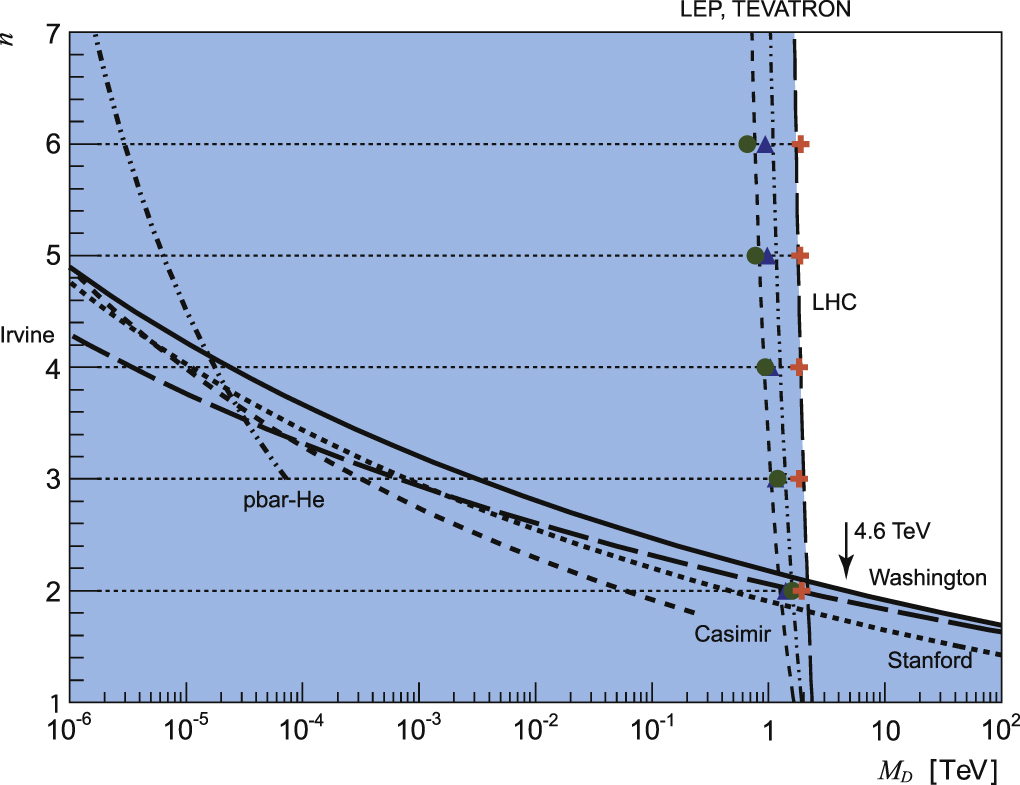
\includegraphics[width=0.90\textwidth]{Figures/add_noncollider_comparison_jpeg.jpg}
    \caption{
      Comparison of collider and noncollider limits on ADD model parameters, as shown in~\cite{ref:0264-9381/32/3/033001}.
      The marked points are monojet limits from the LEP~\cite{ref:9789812702227_0266}, Tevatron~\cite{ref:PhysRevLett.101.181602}, and LHC~\cite{ref:j.physletb.2011.10.006, ref:PhysRevLett.110.011802, ref:0264-9381/32/3/033001}.
      The Irvine~\cite{ref:PhysRevD.32.3084, ref:PhysRevLett.44.1645}, Washington~\cite{ref:PhysRevLett.98.021101}, and Stanford~\cite{ref:PhysRevD.78.022002} curves come from direct measurements of Newton's law.
      The Casimir curve~\cite{ref:0264-9381/32/3/033001} synthesizes of a range of  experimental results that constrain the existence of strong gravity using the Casimir force,
      and the pbar-HE curve~\cite{ref:epjconf/20146605021, ref:0264-9381/32/3/033001} comes from analyses of electron double scattering and exotic atom spectroscopy.
      The ADD model is excluded at 95\% CL or more in the shaded region.
    }
    \label{fig:add_noncollider_comparison}
  \end{center}
\end{figure}

Prior to the analysis presented in this thesis, the most stringent ADD limits in the monophoton final state were set in the last published results from CMS,
based on 12.9 \fbinv\ of data collected in the first half of 2016~\cite{ref:JHEP10(2017)073}. The ADD model was excluded at 95\% CL for $M_\mathrm{D}$ up to 2.31\unit{TeV}
for $n = 3$, climbing to 2.49\unit{TeV} at $n = 6$, as shown in Fig.~\ref{fig:add_cms_earlylimits_MD}.

\begin{figure}[hbtp]
  \begin{center}
    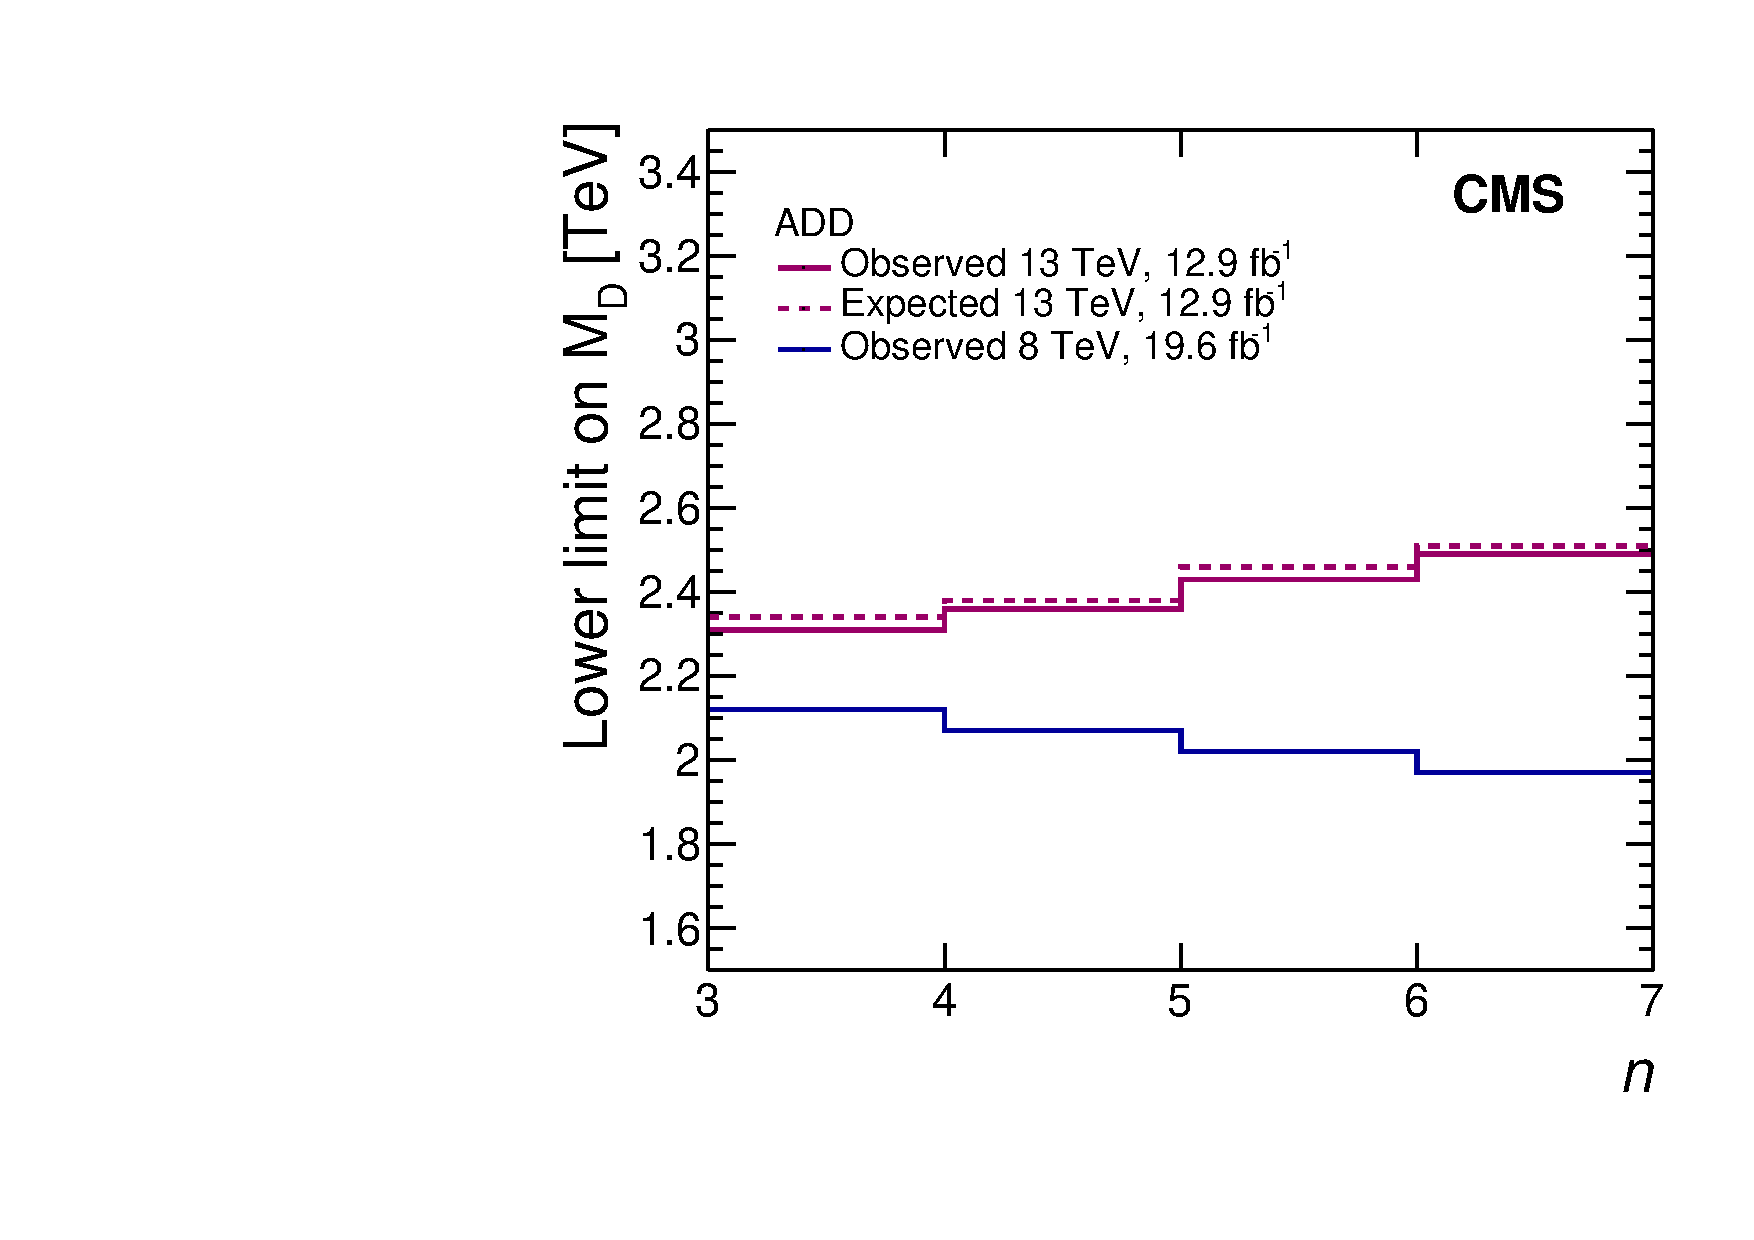
\includegraphics[width=0.50\textwidth]{Figures/add_cms_earlylimits_MD.pdf}
    \caption{
    ADD limits set by the CMS experiment using data from the first half of 2016, as shown in~\cite{ref:JHEP10(2017)073}.
    Limits from the previous CMS analysis of 8\unit{TeV} data~\cite{ref:j.physletb.2016.01.057} are also shown.
    The ADD model for a given $n$ (specified by the left edge of each bin) is excluded at 95\% CL or more for $M_\mathrm{D}$ below the curves.
    }
    \label{fig:add_cms_earlylimits_MD}
  \end{center}
\end{figure}

None of these analyses report any significant evidence of BSM physics.

\chapter{The CMS experiment and the LHC} \label{chap:LHCCMS}
\section{The LHC} \label{sec:LHCCMS_LHC}
The Large Hadron Collider (LHC)~\cite{ref:1748-0221/3/08/S08001} at CERN is, as the name suggests, the world's largest
and most powerful particle accelerator. It is used to collide protons as well as heavy ions, which are both examples of hadrons, hence the ``HC'' in LHC.
Experiments attached to the collider examine the collision debris, from which features of the
parent hard-scattering process may be inferred, allowing models such as those described in Chap.~\ref{chap:introduction} to be tested.

The collider consists of a closed loop of beam pipes, along with its RF cavities (sec.~\ref{sec:LHCCMS_LHC_proton_acceleration}), magnets,
and cryogenic and vacuum systems. It sits in a circular tunnel 26.7\unit{km} in circumference, lying between 45 and 170\unit{m} underground, straddling
the French--Swiss border near Geneva, Switzerland. The beam pipes are subdivided into eight straight and eight arc sections, forming a rounded octagon.
To orient navigation, there are eight designated points spaced evenly around the tunnel perimeter, one in the middle of each 8528\unit{m}-long straight section.
The four main LHC experiments surround the LHC beam pipe at four of these points: ATLAS~\cite{ref:10.1088/1748-0221/3/08/S08003}
at point 1, ALICE~\cite{ref:1748-0221/3/08/S08002} at point 2, CMS~\cite{ref:1748-0221/3/08/S08004} at point 5, and LHCb~\cite{ref:1748-0221/3/08/S08005} at point 8.
Their arrangement is shown in Fig.~\ref{fig:LHC_schematic}.

\begin{figure}[hbtp]
  \begin{center}
    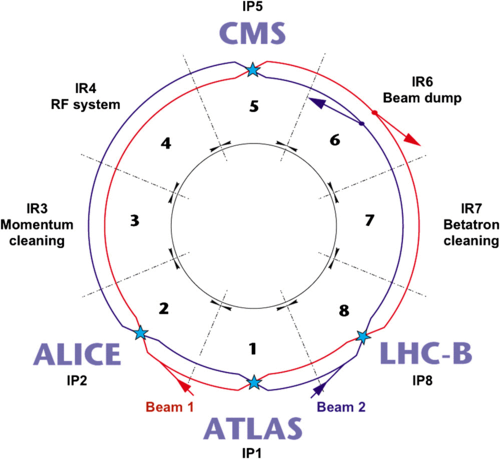
\includegraphics[width=0.70\textwidth]{Figures/Schematic-layout-of-the-LHC-at-CERN.png}
    \caption{
    Schematic layout of the LHC, from~\cite{ref:PhysRevAccelBeams.20.091002}.
    }
    \label{fig:LHC_schematic}
  \end{center}
\end{figure}

The eight arc sections each have a radius of curvature $R = 2.804\unit{km}$. This radius is constrained by the energy of a relativistic particle
bent in a circular trajectory by a magnetic field of magnitude $B$, via the relation~\cite{ref:WilleAccelerators}
\begin{equation}
E = qcBR
\end{equation}
where $q$ is the particle's electric charge and $c$ is the speed of light. For a fixed
particle type and magnet strength, $E$ is directly proportional to $R$. Accordingly, higher-energy
colliders tend to be built with larger circumferences than lower-energy colliders.
The energy of a fully-accelerated LHC proton in 2016 was 6.5\unit{TeV},
corresponding to a bending magnet strength of 7.7\unit{T}.

Smaller accelerators including the Proton Synchrotron (PS) and Super Proton Synchrotron (SPS) used to be flagship accelerators
in their own right, but now chiefly serve as intermediate stages in an accelerator complex that feeds the LHC.
The LHC itself occupies the tunnel originally dug to house the Large Electron-Positron (LEP) collider~\cite{ref:SchopperLEP}, which collided
electrons and their antipartners (positrons) and ran from 1989 until 2000, setting some of the original results
listed in Chap.~\ref{chap:introduction}. The Fermilab Tevatron~\cite{ref:TevatronPhysics}, which ran from 1983 to 2011, occupied a smaller tunnel
but achieved higher energies than LEP by accelerating heavier particles: protons and their antipartners\footnote{These and other recent collider
experiments are reviewed in~\cite{ref:PDG}, chapter 30.}. The LHC, inaugurated in 2008,
accelerates protons in the world's largest accelerator tunnel, with state-of-the-art bending
magnets, allowing it to achieve unprecedented particle collision energies.

\subsection{Proton acceleration and collision} \label{sec:LHCCMS_LHC_proton_acceleration}
The substantial circumference of the LHC beam pipe is compensated by a somewhat narrow width. In practice, a low-energy beam is too wide
to inject directly into the LHC, but the beam can be narrowed by accelerating it.
Furthermore, the beam energy in a specific accelerator of radius $R$ can be tuned by adjusting $B$, but due to the restricted range of
accesible $B$ values for any given magnet~\cite{ref:WilleAccelerators}, a single accelerator can only accommodate a restricted beam energy range.
The beam is therefore passed through multiple accelerators of increasing size before ultimately arriving at the LHC, each of which
increases its energy by an amount commensurate with its radius.
Protons are initially collected by ionizing hydrogen gas and then fed to the LINAC2, a linear accelerator, which accelerates
them to 50\unit{MeV} before sending them to the PS booster, which brings them up to 1.4\unit{GeV}. The protons are then sent to the PS, taking them to 25\unit{GeV},
and after that to the SPS, which pushes them to 450\unit{GeV} before finally injecting them into the LHC for final acceleration
up to 6.5\unit{TeV}.

Protons are accelerated by passing through radio-frequency (RF) cavities, which generate oscillating electromagnetic
fields. Forward acceleration only results if the proton passes through the RF cavity at an opportune point in its oscillation cycle.
Thus, rather than circulating in a continuous beam, protons are segregated into discrete \textit{bunches}. In the LHC, the RF
frequency is tuned to 400.790\unit{MHz}, and bunches are spaced so as to keep 10 RF oscillations between each bunch. This corresponds
to a minimum bunch separation of 24.95\unit{ns} in time, with enough length in the tunnel to fit exactly 3564 bunches, each orbiting
with a frequency $f_\mathrm{rev} = 11.245\unit{kHz}$. A maximum of
2808 bunches can be injected in practice, to allow a sufficiently long empty interval for the beam injection and beam dump
redirector magnets to activate, and also respecting constraints imposed by assembling the bunch trains via the accelerator chain.
Beam optimization strategies and other operational constraints, including a persistent vacuum leak in the SPS beam dump
during 2016, can reduce this further. In 2016, the typical number of bunches per beam $n_b$ was 2076.

Two separate bunch trains counter-rotate around the LHC in separate beam pipes, with their paths crossing at four collision points
corresponding to each of the main experiments. The center-of-mass collision energy of the beams, $\sqrt{s}$, is twice that of the
individual beam energies. For a single-beam energy of 6.5\unit{TeV}, this corresponds to $\sqrt{s} = 13\unit{TeV}$.
Each bunch contains many billions of protons: in 2016, the typical number of protons per bunch at the start of each fill, $N_b$, was $1.25 \times 10^{11}$.
As a consequence, many pairs of protons can undergo hard collisions within the same
bunch crossing, depending on the instantaneous luminosity $\mathcal{L}$ and the total inelastic \Pp\Pp\ scattering cross section $\sigma_\mathrm{inel}$.
In 2016, there were on average 23 of these \textit{pileup} collisions per bunch crossing.

Various parameters describing the geometric profile of the bunches
are listed in Table~\ref{tab:beam_geo}. These determine $\mathcal{L}$ at the collision points, via
\begin{equation}
\mathcal{L} = \frac{N_{b}^{2}n_{b}f_\mathrm{rev}\gamma_{r}}{4\pi\epsilon_{n}\beta^\mathrm{*}}\left(1 + \frac{\theta_{c}^{2}\sigma_{z}^{2}\gamma_{r}}{4\epsilon_{n}\beta^\mathrm{*}}\right)^{-1/2}
\label{eq:instantaneous_lumi}
\end{equation}
in which the relativistic factor $\gamma_{r} = E_\mathrm{beam}/m_{p}$ has a value of 6930 for $E_\mathrm{beam} = 6.5\unit{TeV}$.
The value of $\mathcal{L}$ corresponding to the typical 2016 parameter values listed above is $1.3 \times 10^{34}$ $\mathrm{cm}^{-2}\mathrm{s}^{-1}$.

\begin{table}
\centering
\begin{tabular}{ cc }
\hline
Normalized transverse emittance $\epsilon_{n}$ & 3.4\unit{\micro m} \\
$\beta^{*}$ & 40\unit{cm} \\
Crossing angle $\theta_{c}$ & 185\unit{\micro rad} \\
RMS longitudinal bunch length $\sigma_{z}$ & 7.87\unit{cm} \\
\hline
\end{tabular}
\caption{Beam geometry parameters for 2016}
\label{tab:beam_geo}
\end{table}

\subsection{Collimation, magnets, and beam halo} \label{sec:LHCCMS_LHC_magnets_beam_halo}
The beams can lose protons during transit through a variety of mechanisms, such as intra-beam scattering
and scattering off of residual gas inside the tunnel~\cite{ref:1748-0221/3/08/S08001}. Among other consequences, this leads
to the accumulation of a ``halo'' of protons with large radial separation from the central beam axis, accompanying the main beam.
If left unchecked, beam halo could damage unprotected equipment and leave spurious signals in detectors.
Furthermore, if a bending magnet were to suddenly fail, the beam would sweep across the area downstream of the magnet, dumping a potentially
devastating load of radiation on whatever it hit.

Collimators stationed around the beam line capture and remove this halo,
and additionally protect the LHC and its detectors from sudden beam control failure.
Every proton--collimator interaction produces a residual shower of secondary particles that emerge from the other side of the collimator
and continue forward, so a series of several collimators is required.
Primary LHC collimators (TCP) clean the beam at Points 3 and 7, and secondary collimators (TCS) catch most of the output from those.
Tertiary collimators (TCT) made of a heavy tungsten alloy sit on either side of the CMS experimental cavern,
to scrub as much remaining halo as possible before it reaches the detector~\cite{ref:PhysRevAccelBeams.20.091002}.

As noted above, a charged particle has its trajectory bent as it moves through a magnetic field,
and this principle is used to guide the beams.
A series of 1232 main dipole magnets spaced around the LHC, mostly in the arc regions, keep the beams moving
in their quasi-circular trajectories around the tunnel. A multitude of other magnets serve more specialized roles. Quadrupole
magnets have the effect of squeezing the beam along one axis and stretching it along another, and are used to focus
the beam along a specific direction.
Near the interaction point (IP) of each experiment, an inner triplet of quadrupole magnets
are the last to interact with the beams before they collide. Figure~\ref{fig:magnet_positions} shows the arrangement
of magnets near the ATLAS and CMS IPs.

\begin{figure}[hbtp]
  \begin{center}
    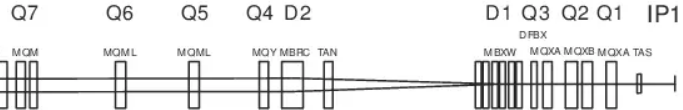
\includegraphics[width=0.80\textwidth]{Figures/magnet_positions.png}
    \caption{
    Dipole (D1-2) and quadrupole (Q1-7) magnet arrangement near the left side of the IP, from~\cite{ref:PAC.2003.1289077}.
    This arrangement is mirrored on the right side of the IP.
    The figure specifically designates IP1, the ATLAS IP; the magnet layout is identical around IP5, the CMS IP.
    The inner triplet of quadrupole magnets (with two varieties, designated MQXA and MQXB)
    are the last to interact with the beam before collision.
    The distance from the left edge of Q3 (MQXA) to the IP is about 53\unit{m},
    and the distance from the right edge of Q1 to the IP is about 23\unit{m}.
    The TCT sits between D2 and TAN, about 150\unit{m} from the IP.
    }
    \label{fig:magnet_positions}
  \end{center}
\end{figure}

The envelope of each beam reaches a maximum in the inner triplet
before finally being focused toward a minimum at the interaction point. Beam halo is correspondingly widely dispersed,
and the TCTs are specifically placed about 150\unit{m} out from the IP so as to protect the inner triplet from this halo~\cite{ref:PhysRevSTAB.18.061001}.
Secondary particles produced from beam
halo collisions with the TCTs include large numbers of high-energy muons, along with an assortment of other secondaries.
These, along with the secondaries from proton collisions with residual gas in the beam pipe, comprise
what is called the machine-induced background (MIB) impinging on CMS~\cite{ref:1748-0221/10/11/P11011}.

In contrast to protons in the beam, secondary muons are neither narrowly nor evenly focused by the final stretch of magnets before reaching the IP.
They enter the CMS cavern traveling parallel to the beam pipe with a wide radial profile, often having a high enough
radius to hit the exterior muon chambers and calorimeters~\cite{ref:1748-0221/10/11/P11011}.
Furthermore, the transverse distribution of MIB (Fig.~\ref{fig:beamhalo_sim}) is highly anisotropic, concentrating near the
horizontal plane.

\begin{figure}[hbtp]
  \begin{center}
    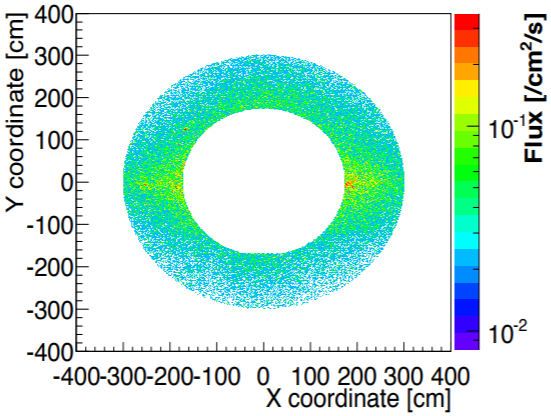
\includegraphics[width=0.50\textwidth]{Figures/beamhalo_sim.png}
    \caption{
    Simulated distribution of MIB flux transverse to the beam pipe in the CMS cavern,
    20.6 m from IP5. From~\cite{ref:1748-0221/10/11/P11011}. The $x$ and $y$ coordinates
    are defined in sec.~\ref{sec:LHCCMS_CMS_coordinates}.
    }
    \label{fig:beamhalo_sim}
  \end{center}
\end{figure}

\section{The CMS experiment} \label{sec:LHCCMS_CMS}
The CMS, short for Compact Muon Solenoid, is a general-purpose particle detector surrounding the LHC beam pipe
centered at IP5, located 100\unit{m} underground near Cessy, France. Multiple layers of metal absorbers, crystal and plastic scintillators,
and electrically-tensed gas chambers and silicon semiconductors are arranged so as to interact with different types of particles in discernably different ways.
Millions of sensors collect fine-grained information on the interactions of particles
within these layers, and the resulting data is used to precisely reconstruct the type, charge, energy, momentum, and trajectory
of nearly every final-state particle emerging from a hard collision event.

A broad overview of the experiment is shown in Fig.~\ref{fig:cms_annotated}.
A more comprehensive description is given in~\cite{ref:1748-0221/3/08/S08004}, the reference from which much of the material in this section derives.
The CMS is a dynamically-evolving apparatus, responding to changing experimental conditions and advances in detection technology and methods.
The description of CMS given in this section specifically applies to its setup in 2016, the year in which collision data for this thesis was taken.

\begin{figure}[hbtp]
  \begin{center}
    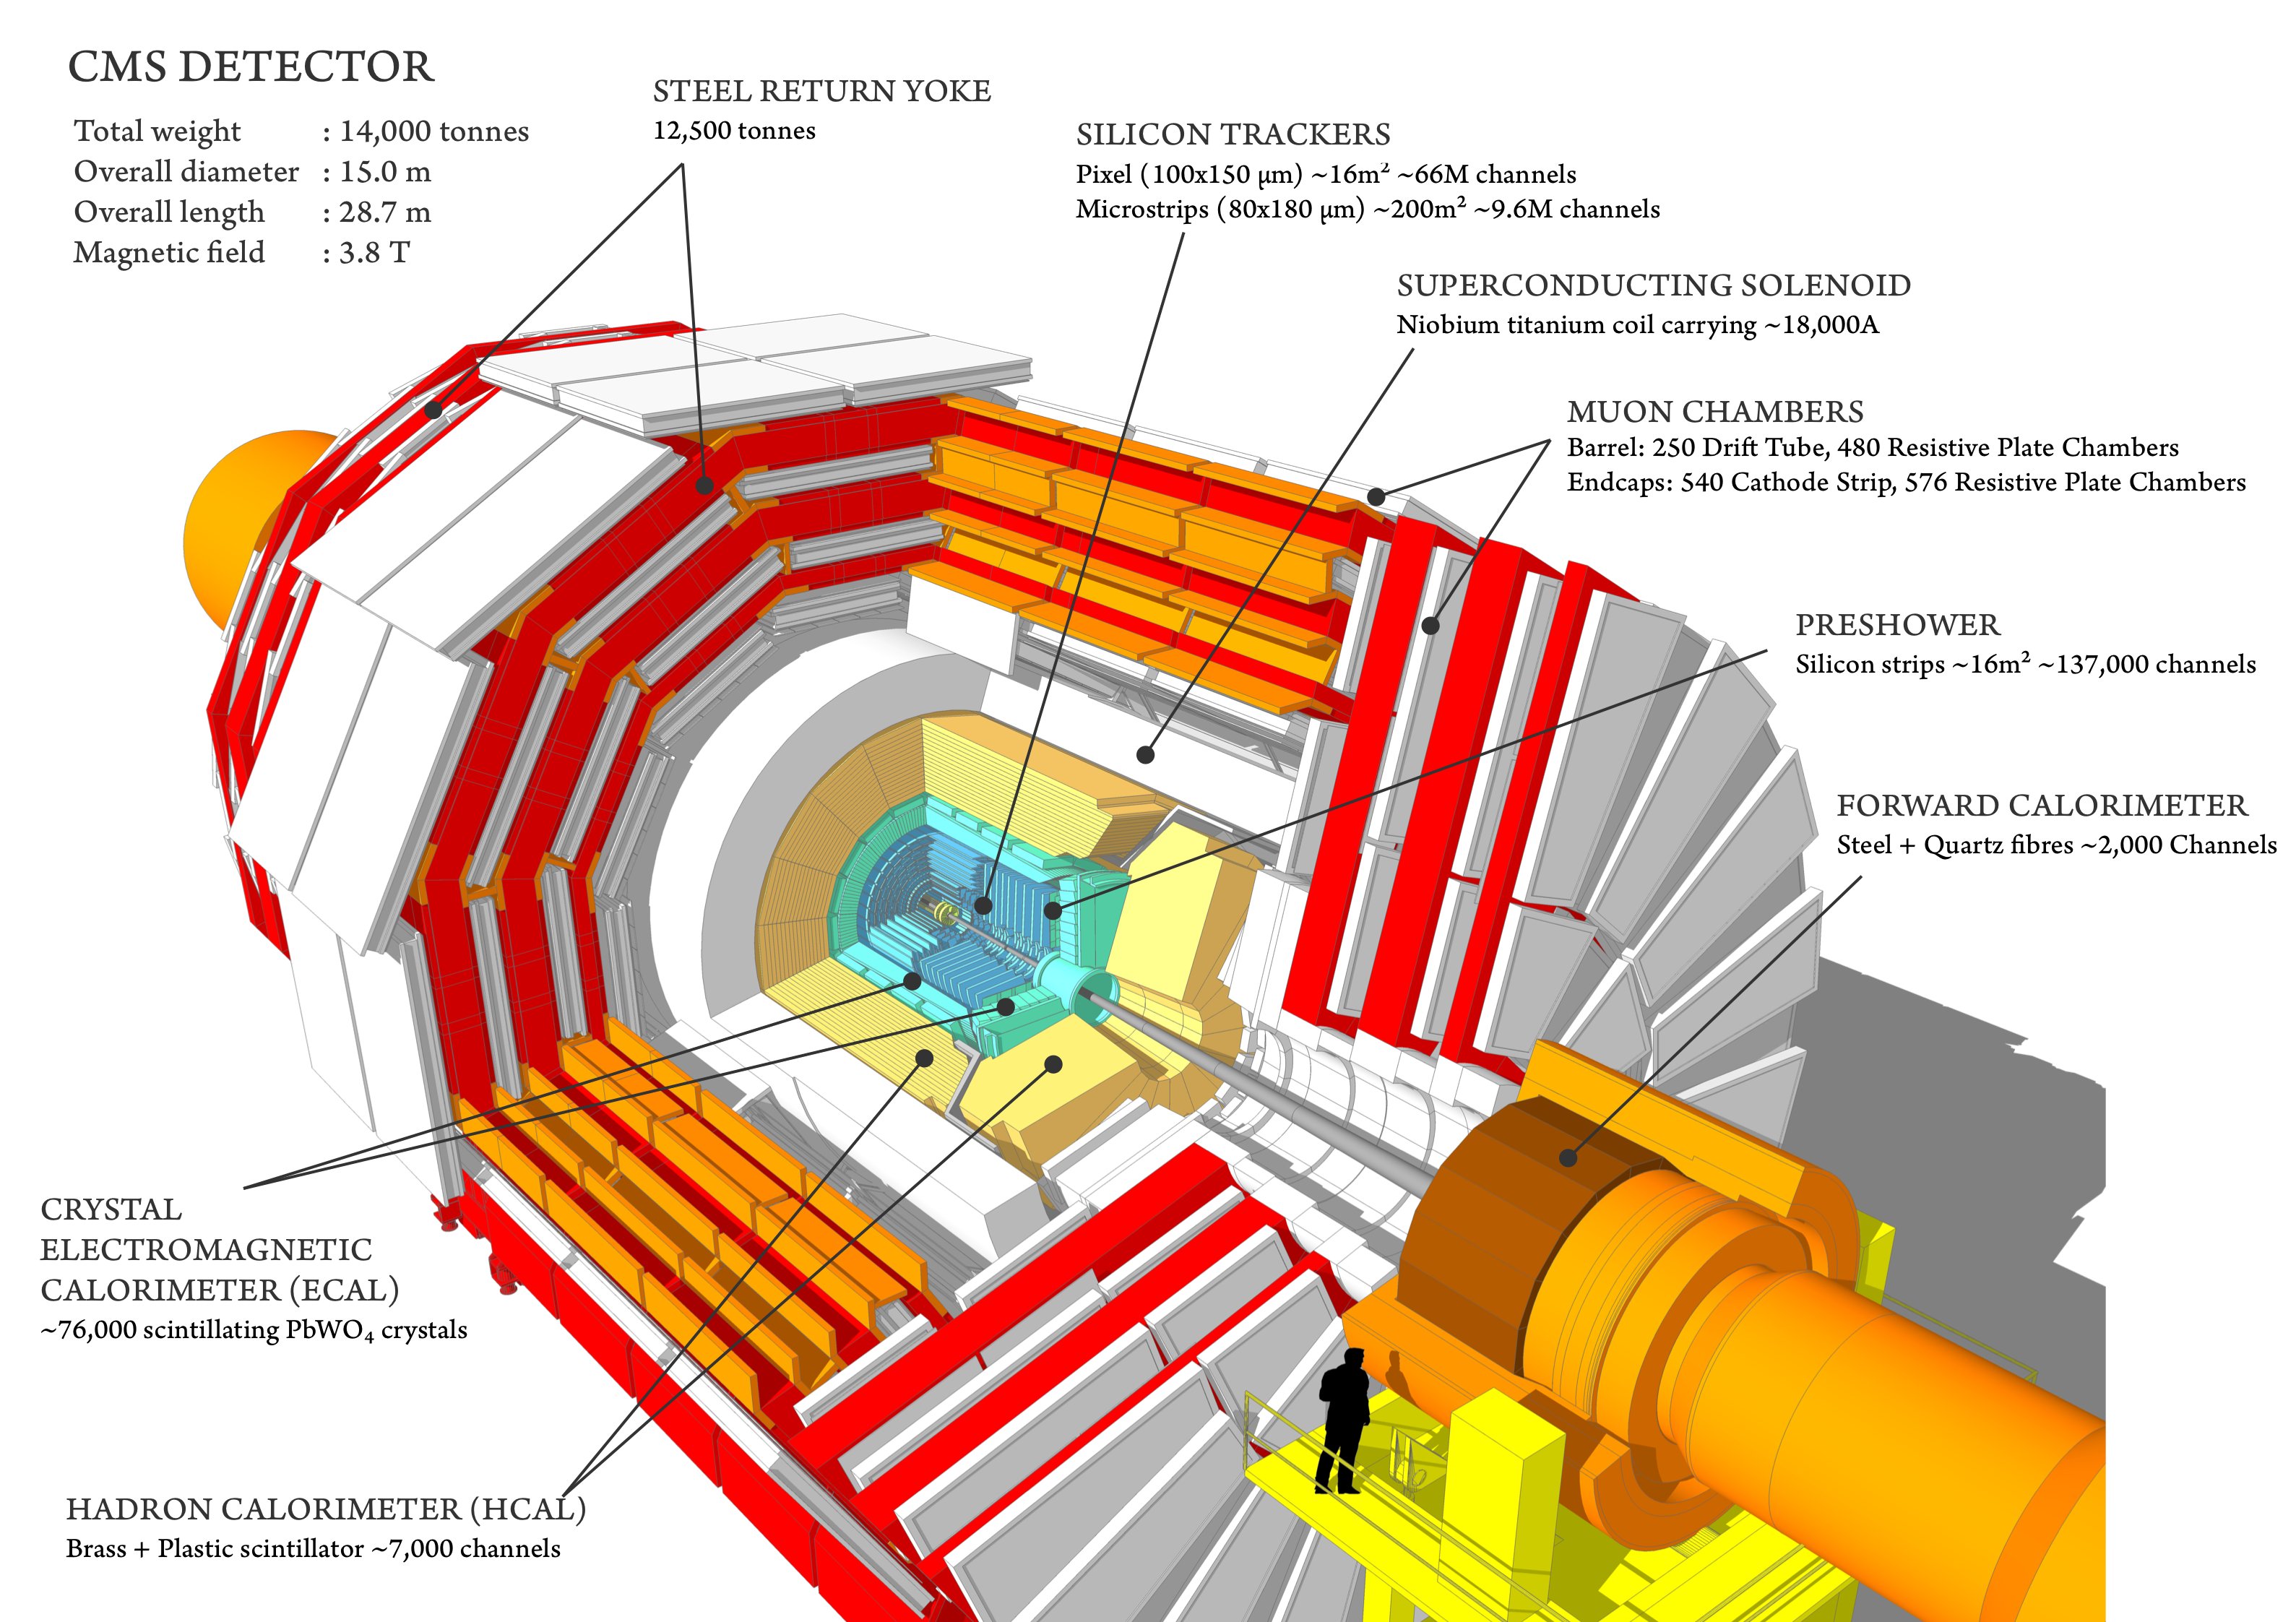
\includegraphics[width=0.99\textwidth]{Figures/cms_annotated.png}
    \caption{
    A schematic illustration of the CMS experiment, with one octant cut away for visibility.
    }
    \label{fig:cms_annotated}
  \end{center}
\end{figure}

\subsection{Coordinate system} \label{sec:LHCCMS_CMS_coordinates}
The coordinate system is centered at IP5, the nominal interaction point inside the CMS experiment.
The positive $x$-direction points radially inward toward the center of the LHC ring, the positive $y$-direction
points vertically upward, and the positive $z$-direction is oriented counterclockwise around the LHC when viewed
from above, as in Fig.~\ref{fig:cms_coordinates}.
The radial coordinate in the $x$--$y$ plane is denoted $r$, and the azimuthal angle $\phi$ is measured counterclockwise
(viewed from the positive $z$-direction, looking toward the negative $z$-direction) from the $x$-axis in this plane.
The polar angle $\theta$ is measured from the positive $z$-direction.

\begin{figure}[hbtp]
  \begin{center}
    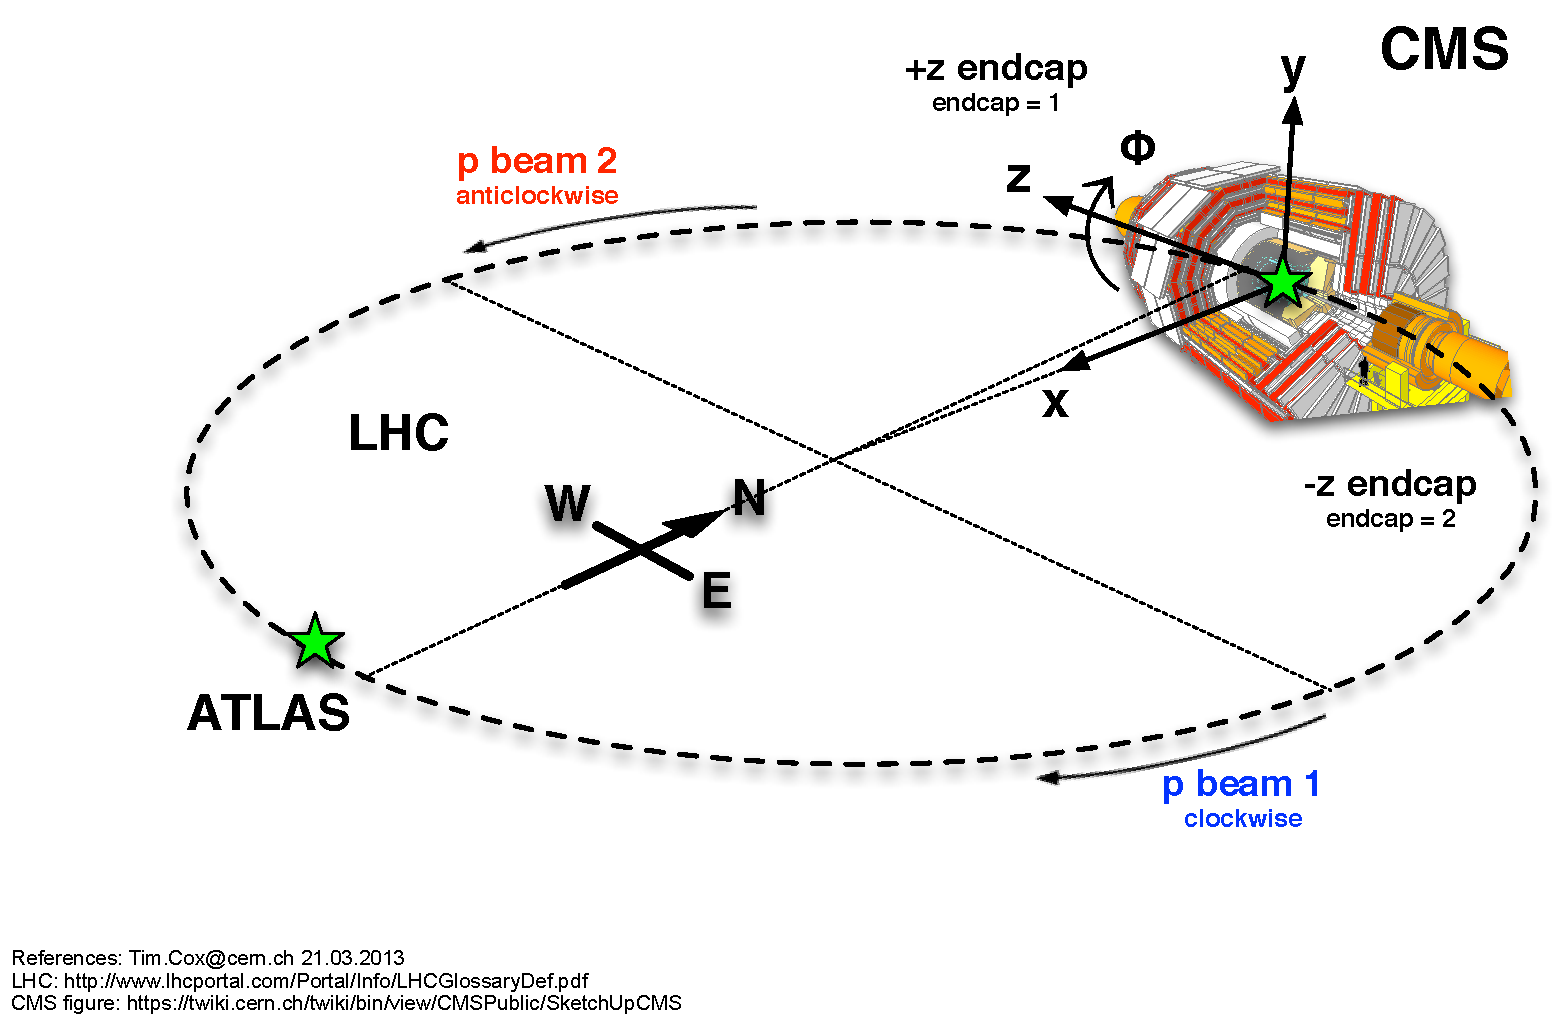
\includegraphics[width=0.90\textwidth]{Figures/cms_coordinates.pdf}
    \caption{
    The CMS coordinate system.
    }
    \label{fig:cms_coordinates}
  \end{center}
\end{figure}

The \textit{longitudinal momentum} of a particle is defined as the component of its momentum along the $z$-axis, with
magnitude $p_\mathrm{L}$. The \textit{transverse momentum} of a particle is the component of its momentum perpendicular
to the longitudinal momentum, lying in the $x$--$y$ plane,
and can be specified by its magnitude \pT\ and its direction $\phi$.

Hard \Pp\Pp\ collisions
result in the interaction of individual partons, each of which can carry different fractions of their
parent \Pp\ momentum. Even if the longitudinal momenta of the colliding protons are perfectly matched,
the longitudinal momenta of the interacting partons may not be. However, the \pT\ of
both parent protons is negligible, and any fraction of zero is still zero. There is some small
\pT\ spread of partons within a proton, but in general, the \pT\ of colliding partons is almost exactly zero, within the limits of detector sensitivity.

By the law of conservation of momentum, the vector sum of the
transverse momenta of all collision products must therefore sum to zero. However, the sum of the longitudinal momenta
can vary appreciably, as can the net longitudinal velocity of the collision event. According
to the theory of special relativity, differences in $\theta$ between events will appear different
to different observers depending on their relative longitudinal velocity. In other words, differences in $\theta$ are not Lorentz invariant.

Differences in a related quantity called the \textit{rapidity}, defined as
\begin{equation}
\mathrm{rapidity} = \frac{1}{2}\ln{\frac{E+p_\mathrm{L}}{E-p_{L}}},
\label{eq:rapidity}
\end{equation}
are Lorentz invariant. Particle production in LHC collisions is roughly constant as a function of rapidity, and because
differences in rapidity do not depend on the longitudinal speed at which one is moving, that statement is independent
of whether the collisions are observed in their own rest frame or in that of the CMS. At very high
energies, rapidity becomes approximatey equal to the \textit{pseudorapidity} $\eta$ defined by
\begin{equation}
\eta = -\ln{\tan{(\theta/2)}}.
\label{eq:pseudorapidity}
\end{equation}

Since $\theta$ only depends on the position of the detector component in which a particle is measured, $\eta$
serves as a convenient coordinate to describe the kinematics of high-energy \Pp\Pp\ collisions in a Lorentz-invariant way.
Pseudorapidity begins at 0 for particles emitted from the IP exactly perpendicular to the beam, and rises in magnitude for particle
trajectories more closely aligned with the beam axis, diverging to infinity as $\theta$ approaches 0.

The CMS has approximately hermetic coverage of particles emerging from the IP with $|\eta|$
up to 5.0, giving a total polar coverage of 178.46 degrees along with complete 360-degree azimuthal coverage. Particles emerging
within this zone of coverage are detected with high probability by at least one subsystem, although the measurement quality varies
as a function of $|\eta|$. Since particles are emitted with a roughly constant concentration as a function of $\eta$, and because
cones of constant $\eta$ become more densely packed at higher values of $|\eta|$, it follows that the intensity of particle radiation
impinging on detector elements is stronger at higher $|\eta|$. Tradeoffs must be made between the measurement quality of an apparatus
and its radiation hardness, and therefore equipment installed at higher $|\eta|$ is typically less precise.

\subsection{Superconducting solenoid and silicon tracking system} \label{sec:LHCCMS_CMS_magnet_tracker}
The ``S'' in CMS derives from the 12.5-m-long, 0.3-m-thick, 6-m-inner diameter solenoid surrounding the core of the experiment.
When an 18 kA current is applied to its more than 2000 windings of superconducting cable, it produces a homogeneous 3.8\unit{T} magnetic
field in its center. The field is returned in the opposite direction with about half the magnitude by an iron return yoke surrounding
the solenoid, consisting of three barrel layers split into five wheels, complemented by three endcap disk layers at each end.

The size and shape of the solenoid are a primary design constraint for CMS. The HCAL, ECAL, and inner tracker together must be compact
enough to fit completely inside it, giving rise to the ``C'' in CMS. Because of the cylindrical shape of the solenoid,
all primary detector layers in CMS are divided into cylindrical barrel sections complemented by flat circular endcaps on either end.

The magnetic field produced by the solenoid is illustrated in Fig.~\ref{fig:solenoid_field}.
Charged particles traveling through this field have their trajectories bent, and at 3.8\unit{T} the field will noticeably
bend even very high-momentum particles. This allows the ratio of a particle's momentum to its charge to be measured, as particles
with higher momentum are bent less than particles with the same charge but lower momentum. It also allows the sign of a particle's electrical charge
to be identified, as positively- and negatively-charged particles are bent in opposite directions (and electrically neutral
particles are not bent at all).

\begin{figure}[hbtp]
  \begin{center}
    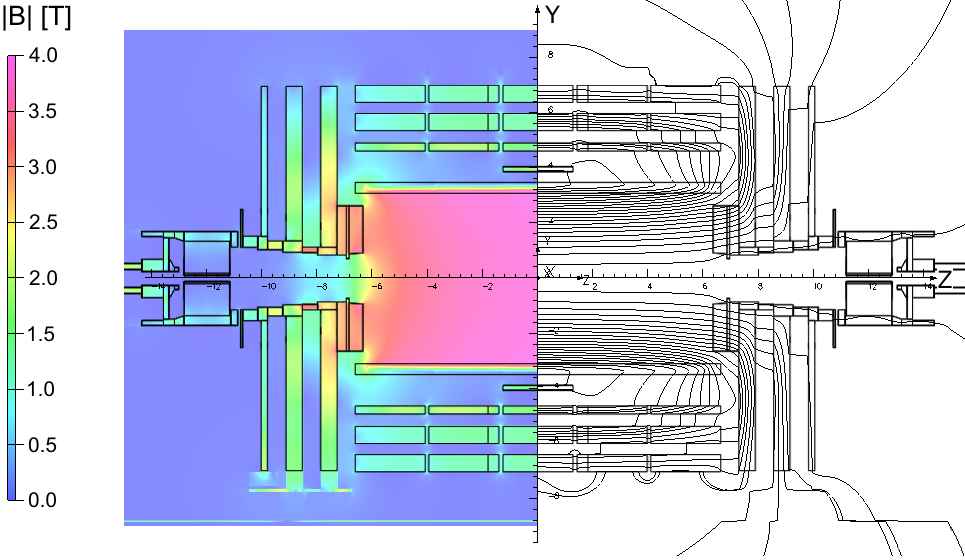
\includegraphics[width=0.90\textwidth]{Figures/solenoid_field.png}
    \caption{
    Magnetic field produced by the CMS solenoid, from~\cite{ref:1748-0221/5/03/T03021}. The field strength in T is shown on the left,
    and contour lines smoothly connecting the field direction are shown on the right.
    }
    \label{fig:solenoid_field}
  \end{center}
\end{figure}

The trajectories of charged particles close to the IP are mapped by an inner silicon tracking system, the innermost detector layer of CMS.
It is based on tracking elements made from radiation-hard silicon, allowing high-speed measurements.
Charged particles passing through the silicon tracker elements release bursts of free electric charge in the silicon. An applied voltage causes
the charge to migrate to a detector at the edge of the element, allowing it to infer the time and location of the hit.
Fine-grained position and time resolution is obtained by subdividing the tracker volume into tens of millions of separate tracking detector elements
spread over multiple layers. Figure~\ref{fig:inner_tracker} illustrates the arrangement of tracker layers.

\begin{figure}[hbtp]
  \begin{center}
    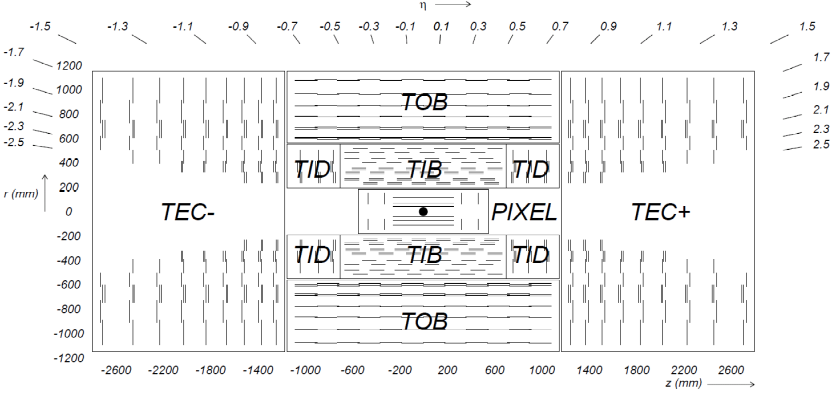
\includegraphics[width=0.99\textwidth]{Figures/tracker_schematic.png}
    \caption{
    Arrangement of layers in the inner tracker.
    }
    \label{fig:inner_tracker}
  \end{center}
\end{figure}

The inner tracker is subdivided into a pixel tracker surrounded by a strip tracker. The pixel tracker is the first CMS module that
low-$|\eta|$ ($\lesssim 2.5$) particles pass through. It is subdivided into three barrel layers at $r = 4.4$, 7.3, and 10.2\unit{cm},
and two endcap disks on each side at $|z| = 34.5$ and 46.5\unit{cm}. These layers are arranged so that at least three are hit by
any particle with $|\eta| < 2.5$.
The tracking elements comprise 66 million pixels, 48 million in the barrel layers
and 18 million in the endcap disks, each with an area of $100{\times}150\unit{\micro m}^{2}$.

The strip tracker is subdivided into an inner barrel (TIB), inner disks (TID), outer barrel (TOB), and endcaps (TEC).
The TIB consists of four cylindrical layers, capped by the TID which comprises three circular disks on each side of TIB.
Together, TIB and TID extend from $r = 20\unit{cm}$ to 50\unit{cm} and out to $|z| = 90\unit{cm}$.
The TOB surrounds the TIB and TID and consists of six cylindrical layers. The TEC caps both TOB and TID and comprises
nine circular disks on each side, complementing the TOB's radial coverage out to $r = 114\unit{cm}$ and extending the $|z|$ coverage
to 280\unit{cm}. The inner radius of TEC tapers upward with increasing radius so as to approximately adhere to the line $|\eta| = 2.5$.
All together, the tracking elements comprise 9.3 million silicon strips, each with an area of $80{\times}180\unit{\micro m}^{2}$.

Both the pixel and strip trackers have hermetic coverage up to $|\eta| = 2.5$. Charged particles with $|\eta|$ in this range will
tend to leave deposits in multiple layers of the inner tracker. By linking these sequential deposits together, the particle's trajectory through the inner
tracker may be inferred.

\subsection{Electromagnetic calorimeter} \label{sec:LHCCMS_CMS_ECAL}
The electromagnetic calorimeter (ECAL) is the second main detector layer, after the inner tracker. It comprises $75\,848$ lead tungstate ($\mathrm{PbWO}_{4}$)
crystals, divided among a cylindrical barrel section (EB) and two endcap sections (EE). The overall structural organization of the ECAL is shown in Fig.~\ref{fig:ecal_schematic}.

\begin{figure}[hbtp]
  \begin{center}
    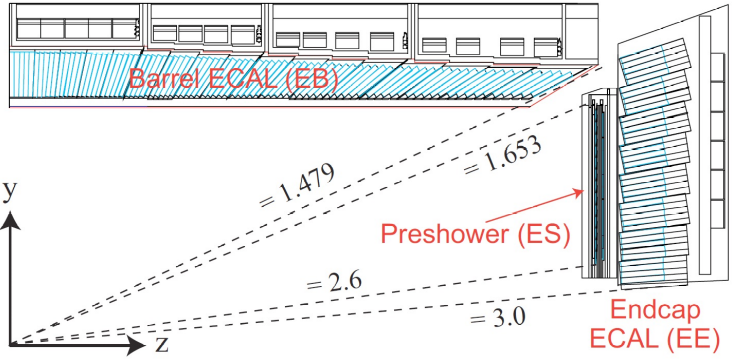
\includegraphics[width=0.80\textwidth]{Figures/ecal_schematic.png}
    \caption{Schematic illustration of the ECAL, showing the longitudinal arrangement of crystals in the barrel and endcap sections.}
    \label{fig:ecal_schematic}
  \end{center}
\end{figure}

The barrel extends to $|\eta| = 1.479$,
and its $61\,200$ crystals are arranged in 170 wheels of 360 crystals each. Every ECAL crystal is shaped like a long, tapered rectangular prism with one
larger, exterior square face attached to a sensor, and a smaller interior square face generally pointing toward the inner tracker. Crystals in EB
are 23.0\unit{cm} long, with a $22{\times}22\unit{mm^2}$ interior face and $26{\times}26\unit{mm^2}$ exterior face. These proportions ensure
a constant coverage of approximately 0.0174 in both $\eta$ and $\phi$ along the entire length of the crystal. The center of each interior face sits at $r = 1.29\unit{m}$.
The crystals lie approximately along projective lines, i.e. lines directed toward the IP. To ensure fully hermetic coverage of particles leaving the IP,
they are tightly packed with 0.35--0.50\unit{mm} of separation between adjacent crystals, and are tilted by 3 degrees off of the true projective line.

The remainder of the ECAL comprises two endcap disks of 7324 crystals each, covering $1.479 < |\eta| < 3.0$.
Crystals in EE are each 22.0\unit{cm} long with a $28.6{\times}28.6\unit{mm^2}$ interior face and $30{\times}30\unit{mm^2}$ exterior face.
The rectangular crystals are stacked in an approximation of a circle. They point along projective lines, directed not at the IP, but rather at a point on
the beam axis 1.3\unit{m} past the IP. The interior edges of EE sit at $|z| = 315.4\unit{cm}$ when the experiment is running\footnote{The intense magnetic
field of the solenoid measurably constricts the CMS detector apparatus, pulling in EE by an estimated 1.6\unit{cm}.}.

Lead tungstate crystal is a scintillator, producing visible
light in the range of 430\unit{nm} (blue-green) in response to the passage of photons and electrons. The blue-green scintillation light travels freely through
the optically transparent crystal, and sensors affixed to the outer face of each crystal collect this light. While its light output is not as high as some other
scintillators (at maximum crystal transparency, about 4.5 electrons per incident MeV are collected by the sensors), $\mathrm{PbWO}_{4}$ was the material of choice
due to its high radiation tolerance, short radiation length ($X_{0} = 0.89\unit{cm}$), and small Molière radius (2.2\unit{cm}).

High-energy electrons (or antielectrons) passing through a high atomic number material such as Pb or W will tend to lose energy in discrete
bursts via the emission of photons (a phenomenon called \textit{bremsstrahlung}, ``braking radiation''), and high-energy photons will tend to propagate freely until suddenly decaying into
an electron--antielectron ($e^{+}e^{-}$) pair. The \textit{radiation length} $X_{0}$ is both the mean distance over which an electron has its energy reduced by bremsstrahlung
by a factor of $1/e$, as well as $7/9$ of the mean free path for photons before they convert to an $e^{+}e^{-}$ pair.

The products of a photon conversion are themselves high-energy electrons and antielectrons, and bremsstrahlung photons tend to have high energies as well,
resulting in a stochastic sequence of photon emissions and $e^{+}e^{-}$ pair production events called an \textit{electromagnetic shower}. As the shower
propagates through a given material, it spreads outward in a roughly conical shape with a characteristic average width. The \textit{Molière radius} of a material
is defined to be the radius of a cylinder, aligned with an electromagnetic shower, encompassing an average of 90\% of the shower's energy.

By conservation of energy, the total shower energy is the same as the energy of the original $e$ or $\gamma$, and by conservation of momentum,
the mean direction of the shower is also the same as that of the original $e/\gamma$. The long depth of the crystals relative to their radiation
length---25.8 $X_{0}$ in EB, 24.7 $X_{0}$ in EE---ensures that nearly 100\% of incident $e/\gamma$ stemming
from \Pp\Pp\ collisions leave electromagnetic showers that are fully contained by the ECAL, allowing their energies to be reliably inferred.
The small Molière radius of $\mathrm{PbWO}_{4}$ allows their orientation to be accurately judged, and nearby showers can be reliably separated in most cases.

The scintillation light is collected in EB crystals by avalanche photodiodes (APDs), and in EE crystals by more radiation-tolerant
vacuum phototriodes (VPT). The amount of light collected is directly proportional to the shower energy contained in the crystal.
The time of arrival of the shower is inferred by fitting a pulse shape to input signals collected every 25\unit{ns}. It takes time for the
crystal scintillation to fully die down---after 25\unit{ns}, about 80\% of the total scintillation light has been emitted---so the full pulse shape
is spread over more than one input.

Free neutrons produced in the calorimeters can migrate through the detector and interact with a layer of epoxy used to affix the APD
to the crystal surface, ejecting protons directly into the APD active volume. This triggers the release of thousands of electrons into the APD,
resulting in a spurious signal that can be mistakenly reconstructed as an $e/\gamma$ deposit with very high energy~\cite{ref:1742-6596/404/1/012043}.
Since these \textit{spikes} occur in single crystals, most can be distinguished from real $e/\gamma$ showers by their narrow distribution of shower energy,
as illustrated in Fig.~\ref{fig:spike_energy_distribution}.
The APD does not receive a continuous light signal from the crystal scintillation in these events, so the pulse shape is constructed from
only one input signal, as illustrated in Fig.~\ref{fig:spike_pulse_shape}. This has the net effect of shifting the inferred time of arrival backward, and most spikes have a measured arrival time between 10 and 15\unit{ns}
before real photons in a given bunch crossing. ``Double spikes'' involving two neighboring crystals have also been observed, presumably
arising from a secondary nucleon ejected by the primary neutron. These are similarly distinguishable from real $e/\gamma$ showers by their narrow
energy distribution and early arrival time.

\begin{figure}[hbtp]
  \begin{center}
    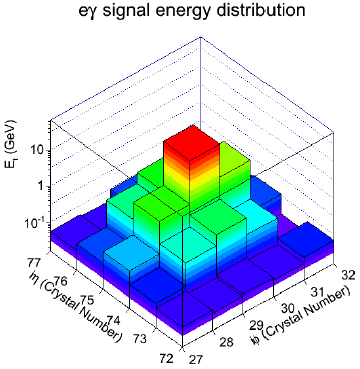
\includegraphics[width=0.49\textwidth]{Figures/real_egamma_energy_distribution.png}
    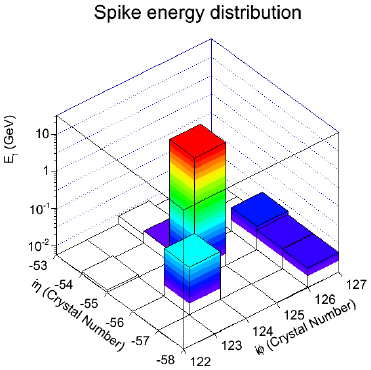
\includegraphics[width=0.49\textwidth]{Figures/spike_energy_distribution.png}
    \caption{Distributions of electromagnetic shower energy among neighboring ECAL crystals. The distribution from an actual
    $e/\gamma$ shower is shown on the left, and a spike distribution is shown on the right. From~\cite{ref:spikes_farzanehfar}.}
    \label{fig:spike_energy_distribution}
  \end{center}
\end{figure}

\begin{figure}[hbtp]
  \begin{center}
    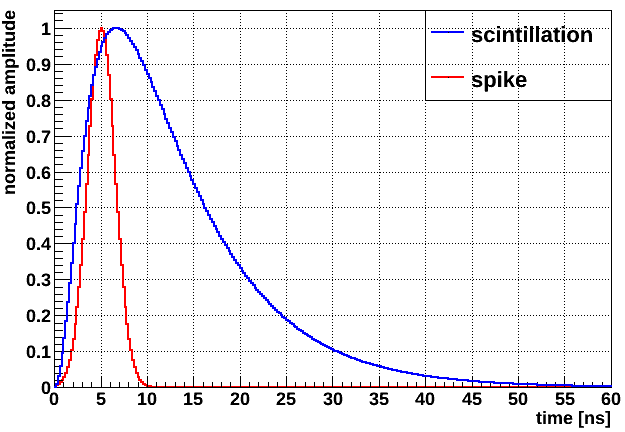
\includegraphics[width=0.60\textwidth]{Figures/spike_pulse.png}
    \caption{Pulse shapes in the APD produced by spikes and by genuine electromagnetic showers, from~\cite{ref:DN-2015/014}.}
    \label{fig:spike_pulse_shape}
  \end{center}
\end{figure}

Neutral pions (a type of hadron produced copiously in \Pp\Pp\ collisions) decay rapidly into two photons,
and when the pion is traveling at high speed, these photons will emerge moving in very close to the same direction.
Despite the relatively small Molière radius of $\mathrm{PbWO}_{4}$, it can still be difficult to discern whether the ECAL
has been struck by a single high-energy photon or two tightly-collimated photons from a pion decay.
To facilitate the identification of these pions, a preshower detector is installed on the EE.

The preshower comprises two modules, one attached to the inner edge of each ECAL endcap. A module consists of two layers,
each with a lead radiator followed by a silicon strip sensor, and has a total thickness of 20\unit{cm}, covering $1.653 < |\eta| < 2.6$.
The inner lead layer initiates electromagnetic showers from incoming $e/\gamma$ particles,
and the silicon sensor behind it measures the shower shape and energy.
The second layer of lead continues the shower evolution, and the second layer of sensors provides another measurement.
This is an example of a sampling calorimeter, and the same general strategy is employed by HCAL, described in the following section.

\subsection{Hadronic calorimeter} \label{sec:LHCCMS_CMS_HCAL}
After the ECAL, the next layer a particle will encounter is the hadron calorimeter (HCAL)\footnote{If the particle has $|\eta| > 3.0$,
the forward portion of HCAL is the first and only CMS detector layer it hits.}.
The HCAL is subdivided into three main systems: the barrel (HB), endcap (HE), and forward calorimeters (HF).
Figure~\ref{fig:hcal_schematic} shows their overall layout.

\begin{figure}[hbtp]
  \begin{center}
    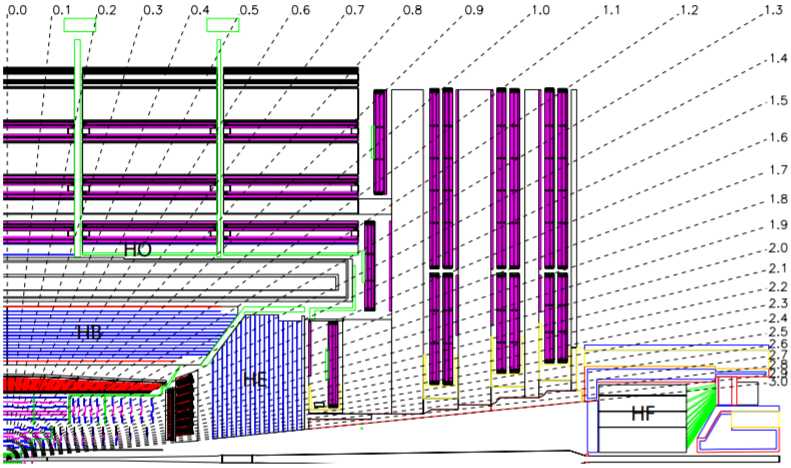
\includegraphics[width=0.90\textwidth]{Figures/hcal_layout.png}
    \caption{
    Schematic illustration of the HCAL overlaid with dashed lines of constant $\eta$, from~\cite{ref:1748-0221/3/08/S08004}.
    Indicative arrangements of the muon systems, solenoid, ECAL, and inner tracker are also shown.
    }
    \label{fig:hcal_schematic}
  \end{center}
\end{figure}

The barrel and endcap systems are sampling calorimeters with alternating layers of brass absorber and plastic scintillator.
The brass in the absorbers is an alloy of 70\% Cu and 30\% Zn. High-energy hadrons hitting the nuclei in these atoms can eject
a number of secondary hadrons, which themselves can eject further hadrons in a cascade known as a \textit{hadronic shower}.
Like electromagnetic showers, hadronic showers have a characteristic length, the \textit{nuclear interaction length} $\lambda_{I}$.
Hadrons such as pions can also decay midflight into high-energy $e/\gamma$, leading to secondary electromagnetic showers.
The brass absorbers have $\lambda_{I} = 16.42\unit{cm}$ and $X_{0} = 1.49\unit{cm}$.

Absorber layers are interleaved with plastic scintillator tiles, with about 70\,000 in total distributed between HB and HE.
Inlaid fiber optic cables sample the scintillation light and carry it to hybrid photodiode (HPD) sensors. Up to 17 layers of
plastic scintillator are stacked against each other in HB and HE, interleaved by brass absorber layers.

The barrel section covers $|\eta| < 1.3$.
Layers of HCAL scintillators and absorbers lie parallel to the beam line. Towers of related scintillator tiles are grouped along
projective lines pointing toward the IP, as shown in Fig.~\ref{fig:hcal_towers}.
In HB there are 16 tower divisions in $\eta$ on either side of $\eta = 0$, and 72 tower divisions in $\phi$, such that each tower
has an $\eta$--$\phi$ coverage of $0.087{\times}0.087$. The brass and scintillator layers are separated into wedges in $\phi$.
So as to ensure hermetic coverage throughout HB, the brass layers within each wedge are staggered, and adjacent wedges are separated by less than 2\unit{mm}.

\begin{figure}[hbtp]
  \begin{center}
    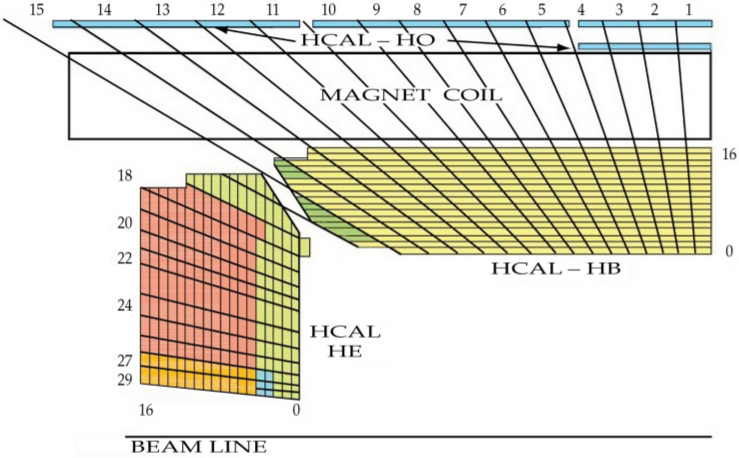
\includegraphics[width=0.75\textwidth]{Figures/hcal_towers.png}
    \caption{
    Arrangement of HB, HE, and HO towers, from~\cite{ref:1748-0221/3/08/S08004}.
    }
    \label{fig:hcal_towers}
  \end{center}
\end{figure}

The effective thickness of HB ranges from 5.39 $\lambda_{I}$ at tower 0 to 10.3 $\lambda_{I}$ at tower 15; tower 16 partially overlaps with HE.
About 1.1 additional $\lambda_{I}$ are supplied by the ECAL. The thickness of HB is constrained by the available space between EB
and the solenoid. In order to provide a more robust measurement of shower energy, and also to supply additional insulation to the outer muon systems
by capturing hadrons exiting the rear of HB, HCAL is supplemented by an outer barrel layer (HO) directly behind the solenoid.
The solenoid itself contributes about 1.4 $\lambda_{I}$ at low $|\eta|$.

The endcaps cover $1.3 < |\eta| < 3.0$. Like HB, the layers in HE are staggered so as to provide hermetic coverage. Unlike HB,
no additional outer layer is needed, since HE is about 10 $\lambda_{I}$ thick over its entire span. Towers in EE have a coverage
of $0.087{\times}0.087$ for $|\eta| < 1.6$ and approximately $0.17{\times}0.17$ for $1.6 < |\eta| < 3$.

The HF covers the forward region, $3 < |\eta| < 5$. It is composed mostly of steel with embedded quartz fiber, built in a cylindrical shape with a radius of 130.0\unit{cm}.
The cylinder's inner face sits 11.2\unit{m} from the IP and it extends 165\unit{cm} longitudinally, supplying approximately 10 $\lambda_{I}$ for
the development of hadronic showers. The intense radiation in the forward region necessitated the use of quartz fibers as the active medium for shower energy probing.
High-energy charged particles in these showers generate Cherenkov light as they pass through the fibers, which run from front to back through the cylinder,
and serve as fiber optic cables carrying that light to photomultiplier tubes. Half of the fibers run over the full length of the
steel cylinder, and the other half begin 22\unit{cm} back from the inner face, allowing $e/\gamma$ (which deposit most of their energy in the first 22\unit{cm}) to be
distinguished from hadrons (which deposit their energy roughly equally before and after 22\unit{cm}). The fibers are bundled in towers, each with an
$\eta$--$\phi$ coverage of $0.175{\times}0.175$. For additional radiation protection, the HF is enclosed by layers of steel, concrete, and polyethylene shielding,
up to 85\unit{cm} thick on the sides.

\subsection{Muon systems} \label{sec:LHCCMS_CMS_muon}
The ``M'' in CMS reflects the central role of muon detection and measurement in the design of the experiment.
High-energy muons are minimum-ionizing particles (MIPs), reaching the outer muon systems largely unaffected by their passage through
the inner detector layers. In contrast, most other particles are fully absorbed by more than 16 $\lambda_{I}$ of material in the inner
layers, leaving a relatively background-free environment in the muon chambers.

The muon chambers interleave the steel flux-return yoke, which in addition to concentrating the exterior magnetic field also serves
to block other remnant particles from reaching the chambers. The layout of muon chambers is shown in Fig.~\ref{fig:muon_system}.
Like other CMS layers, the muon system is divided into a central barrel section and two endcaps. The barrel section is instrumented by four
layers of drift tube (DT) chambers, which cover $|\eta| < 1.2$. Each layer contains 8 chambers that measure the muon coordinates in the $r$--$\phi$
plane, and the inner three layers have an additional 4 chambers to measure the muon coordinate in the $z$ axis.

\begin{figure}[hbtp]
  \begin{center}
    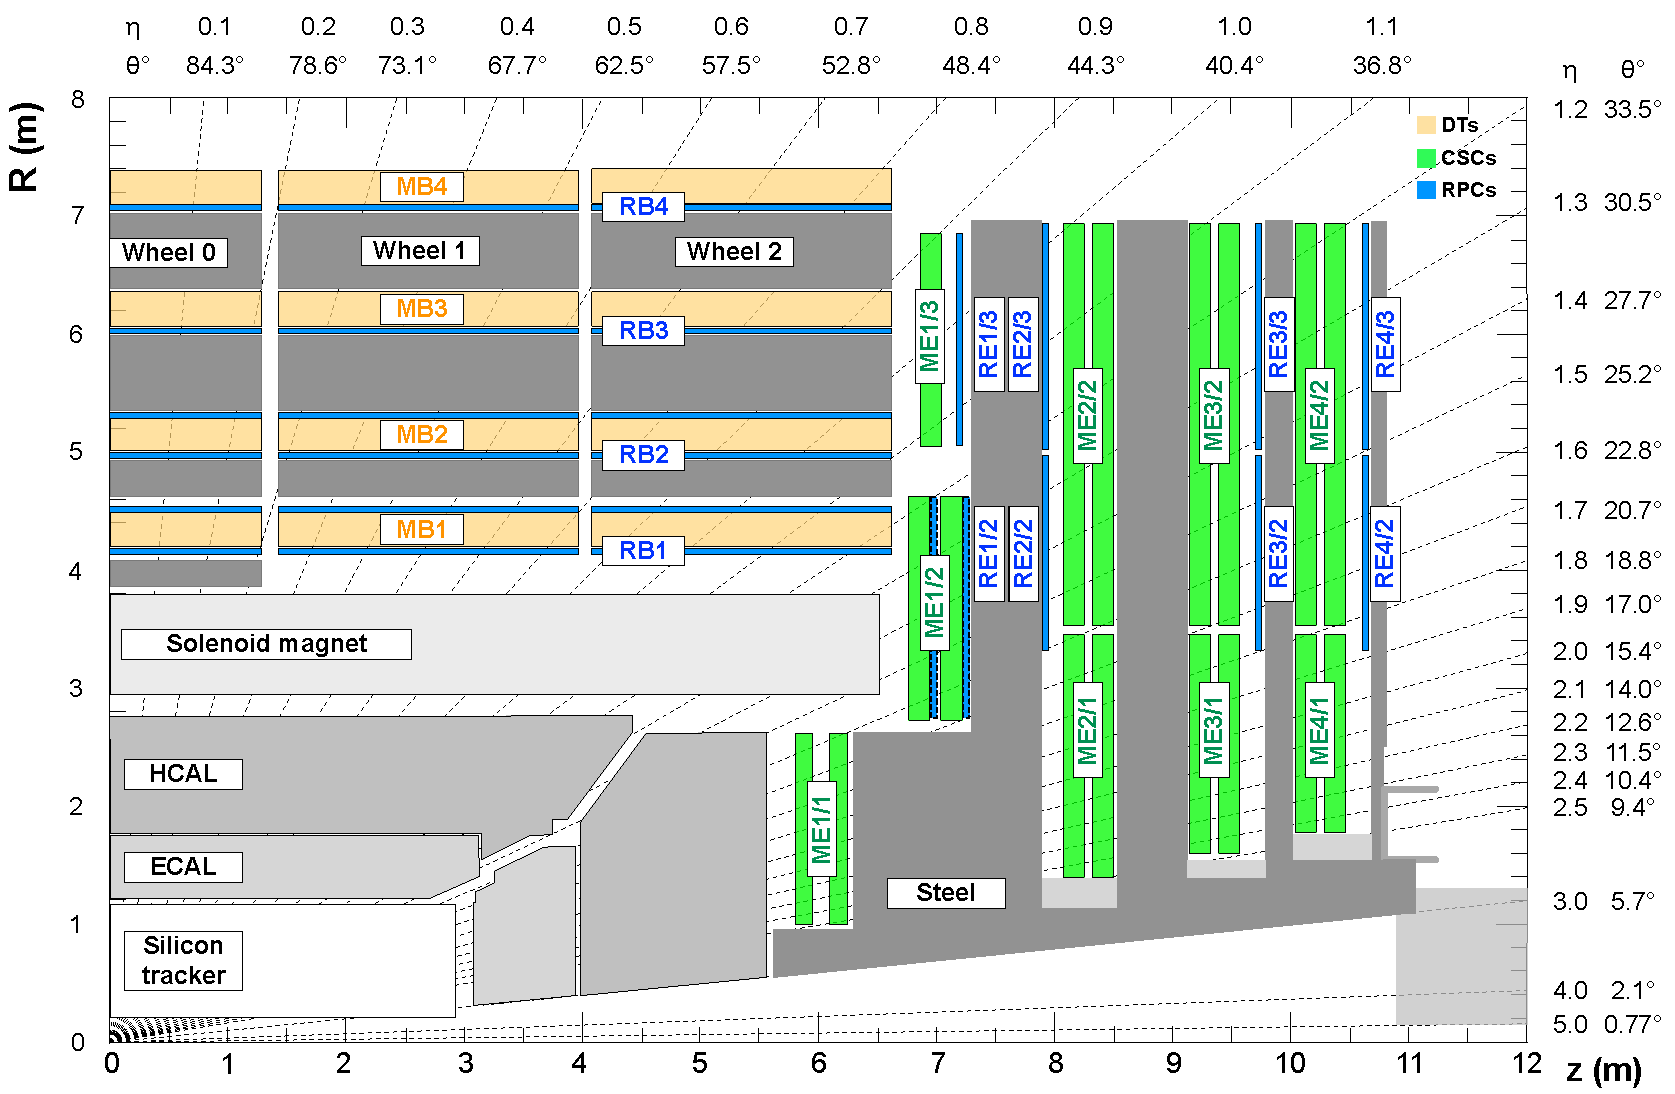
\includegraphics[width=0.99\textwidth]{Figures/muon_system.pdf}
    \caption{
    Muon systems in a quadrant of CMS. Indicative arrangements of the solenoid, HCAL, ECAL, and inner
    tracker are also shown.
    }
    \label{fig:muon_system}
  \end{center}
\end{figure}

The endcaps, subject to higher radiation fluences and more nonuniform magnetic fields, are instrumented by four layers of cathode strip chambers (CSCs),
which cover $0.9 < |\eta| < 2.4$. Cathode strips, oriented in the radial direction, give a measurement in the $r$--$\phi$ plane, and anode
wires running perpendicular to the strips provide an additional measurement of the muon $\eta$.

During the design of CMS, the reliability of time measurements from these two systems of muon chambers was highly uncertain, and thus a third system
consisting of resistive plate chambers (RPCs) was installed. These provide a relatively coarse position measurement, but a highly
accurate time measurement. Muons with $|\eta|$ up to about 1.7 will pass through at least 4 RPC layers.

\subsection{Trigger system} \label{sec:LHCCMS_CMS_trigger}
Data readout from the detectors occurs at a rate of 40\unit{MHz} (once every 25\unit{ns}), corresponding with the LHC bunch crossing frequency.
The memory needed to store the full data produced in one collision event is about 1\unit{MB}, and
it is presently impossible to extract or store data collected at a rate of 40 million \unit{MB/s}.
Therefore, the data is first filtered through a \textit{trigger} system, which rapidly decides which events to store
and which to discard.

The trigger system proceeds in sequential levels. The Level 1 (L1) trigger uses a reduced set of detector information to make an initial,
extremely rapid (within 4\unit{\micro s}) filtering decision at the rate of 100\unit{kHz}. Meanwhile the full detector data sits in a buffer.
If the L1 accept (L1A) is given, that data is sent to the High-Level Trigger (HLT); otherwise it is discarded.
The HLT uses the full data to make a less time-intensive, more sophisticated decision. Events accepted by the HLT have their data permanently stored.

The L1 trigger consists of custom hardware connected by fiber links to the CMS muon and calorimeter systems\footnote{Information
from the inner tracker is not presently used by L1.}. Information from HCAL and ECAL is
sent through a dedicated calorimeter trigger pipeline, and information from the muon systems is sent through a separate muon trigger pipeline.
The output of both of these pipelines is evaluated by a Global Trigger (GT), which makes
the final L1A decision. The organization of L1 pipelines is illustrated in Fig.~\ref{fig:l1_trigger_pipeline}.

\begin{figure}[hbtp]
  \begin{center}
    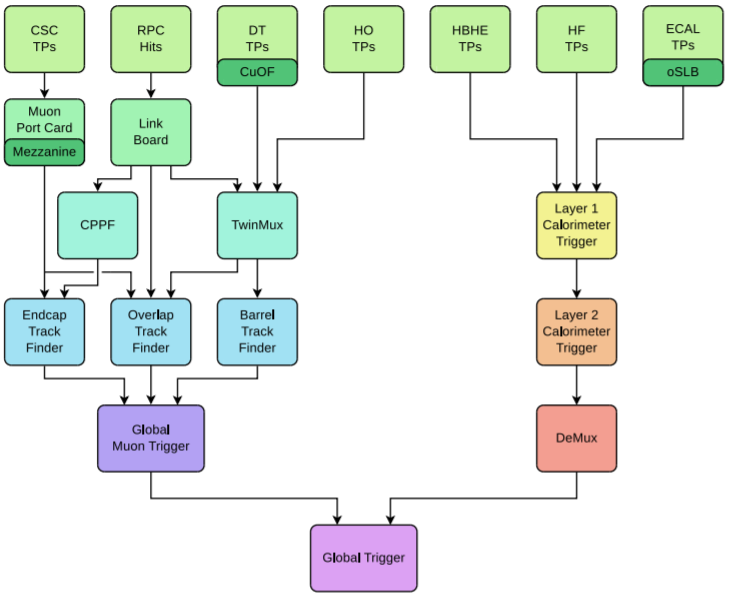
\includegraphics[width=0.80\textwidth]{Figures/l1_trigger_pipeline.png}
    \caption{
    Schematic diagram of the L1 trigger pipeline.
    }
    \label{fig:l1_trigger_pipeline}
  \end{center}
\end{figure}

The \textit{trigger primitives} (TPs) sent by HCAL and ECAL are transverse energy sums recorded in calorimeter towers.
These along with some quality information are sent to Layer 1 of the calorimeter trigger,
which performs preprocessing, energy calibration, and the computation of some simple values. Layer 2 uses this information to construct
various physics objects---L1 Jets, Taus, and EGamma\footnote{With only calorimeter information, it is difficult to distinguish $e$ from $\gamma$.
In full offline event reconstruction, this classification is refined by incorporating inner tracker information.}---using simple and fast reconstruction algorithms.
Layer 2 comprises 9 parallel cards which analyze sequential events in a round-robin, ``time-multiplexed'' fashion, so as to give
each card adequate memory and processing time for each event. The demultiplexer (DeMux) organizes the resulting output and sorts the L1 objects by $p_\mathrm{T}$,
sending this information along to the GT.

The TPs from CSCs and DTs are track segments. Along with hits recorded in the RPCs, muon system TPs are routed through a lattice of preprocessor
layers and then sent to dedicated Barrel, Endcap, and Overlap Track Finders covering different $\eta$ regions.
These rapidly assemble L1 Muon objects and send them to the Global Muon Trigger,
which sorts the L1 Muons by $p_\mathrm{T}$ and quality, finally sending this information along to the GT.

The GT tests the L1 objects it receives against a set of L1 trigger paths, which specify various event selection criteria. After evaluating
which trigger paths have been passed, the GT makes the final L1A decision. The time from TP generation to L1A decision cannot be longer than
4\unit{\micro s}, and the overall L1A rate cannot be higher than 100\unit{kHz}; in 2016, this was the typical L1A rate actually achieved.

If the L1A is given, the full detector data is sent to the HLT, which consists of software running on commercial computing hardware.
The HLT tests each event against a set of high-level trigger paths. Each of these paths has access to raw detector information as well
as quantities computed at L1. Enough time and memory are available to perform a reduced sequence of the full offline event reconstruction
algorithms, separately optimized for each path. In 2016, the average HLT processing time per event was less than 160\unit{ms},
and the typical HLT accept rate was 1\unit{kHz}.

\subsection{Luminosity measurement} \label{sec:LHCCMS_CMS_lumi}
In principle, the integrated luminosity is given by integrating the instantaneous luminosity defined by Eq.~\ref{eq:instantaneous_lumi} over the data taking period,
with an extra efficiency factor to account for the fraction of time during which the trigger was active. In practice, the uncertainty on the
parameters of Eq.~\ref{eq:instantaneous_lumi} is fairly high, and more precise measurements of instantaneous luminosity are obtained by directly examining the beam intensities.

In the method developed
by van der Meer~\cite{ref:CERN-ISR-PO-68-31}, the two beams are scanned across each other in the transverse plane, giving a direct experimental
probe of the beam profile that is used to calibrate the relationship between instantaneous luminosity and specific observables accessible to various
beam monitoring instruments. A van der Meer scan establishes the calibrated visible cross section $\sigma_\mathrm{vis}$ of a process examined
by each luminometer, such that the instantaneous luminosity measured by a luminometer is given by
\begin{equation}
\mathcal{L} = R / \sigma_\mathrm{vis}
\label{eq:lumi_calibration}
\end{equation}
where $R$ is the observed rate of the process measured by the luminometer. The pixel tracker, DTs, and HF are used for this purpose, in addition to two
dedicated instruments: the Fast Beam Conditions Monitor (BCM1f) and Pixel Luminosity Telescope (PLT).

Van der Meer scans require dedicated LHC runs outside of normal data taking, but the calibrated luminometers continue to monitor the beam luminosity
during physics runs. The uncertainty on calibrated luminosity measurements in 2016 data taking is 2.5\%~\cite{ref:CMS-PAS-LUM-17-001}.
The data set used in this thesis corresponds to a time-integrated luminosity $L = 35.9$ \fbinv.

\chapter{Simulation} \label{chap:simulation}
\section{Parton distribution functions} \label{sec:simulation_pdf}
A hard collision involving a proton can cause individual partons within it to be clearly resolved.
For collisions with characteristic energy $Q$, the probability that the parton will be of type $i$
and carry a fraction $x$ of the proton's total momentum is given by a function $f_{i}(x, Q^{2})$
known as a parton distribution function (PDF).

The dependence of these functions on $Q$ is described by the DGLAP equations~\cite{ref:0370-2693(71)90576-4, ref:dokshitzer, ref:0550-3213(77)90384-4},
which are derived from the theory of QCD.
These allow the specific values of $f_{i}(x, Q^{2})$ to be calculated at arbitrary $Q$ as long as they
are first measured at some particular $Q$.
Like cross sections, the DGLAP equations, and hence PDFs derived in this way, admit perturbative expansions out to specific orders in
$\alpha_\mathrm{S}$~\cite{ref:0034-4885/70/1/R02}.

Simulated samples used in this thesis use PDFs computed to different orders as appropriate for the order
of the cross section used. Samples with cross sections computed to LO in $\alpha_\mathrm{S}$ use the NNPDF3.0 LO PDF
set~\cite{ref:NNPDF30}. Samples with NLO cross sections, as well as theoretical \zinvg, \wlng, and \zllg\ cross sections
computed to NNLO in MATRIX, use the NNPDF3.1 NNLO PDF set~\cite{ref:NNPDF31}.
These PDF sets are based on fits of the theoretical DGLAP functional form to the experimentally-measured values
of the PDFs from multiple experiments, examining a variety of processes at a range of different energy scales.

\section{Hard process generation} \label{sec:simulation_hard_process}
A generic hard proton scattering process proceeds as
\begin{equation}
\Pp + \Pp \to X + rest
\end{equation}
where $X$ is a high-energy final product (such as a \Pgamma) of a hard parton--parton collision, and $rest$ is a collection of
lower-energy final-state hadrons emerging from softer parton interactions.

According to the QCD factorization theorem, the dominant contribution to the cross section $\sigma_{X}$ of such a process is given by (see e.g.~\cite{ref:BargerPhillips})
\begin{equation}
\sigma_{X} = \sum_{i,j}\int \! dx_{1}dx_{2} \, f_{i}(x_{1}, \mu_{F}^{2})f_{j}(x_{2}, \mu_{F}^{2})\sigma_{i,j \to X}
\end{equation}
where $i,j$ specify the types of the hard scattering partons, and $\sigma_{i,j \to X}$ is the cross section for the partonic process
\begin{equation}
i + j \to X + rest
\end{equation}
which can be computed to a desired order using Feynman diagrams\footnote{Here $rest$ is a collection of quarks and gluons
that eventually fragment into final-state hadrons.}. The energy scale $\mu_{F}$ is called the factorization scale.
The value of $\alpha_\mathrm{S}$, which appears in perturbative expansions of $\sigma_{i,j \to X}$, is governed by another energy scale $\mu_{R}$ called
the renormalization scale\footnote{As the characteristic
energy scale increases, the effective value of $\alpha_\mathrm{S}$ decreases. This is in contrast to the fine structure ``constant'' $\alpha$,
whose value increases with increasing energy.}.
The coefficients of $\alpha_\mathrm{S}$ in such perturbative expansions also depend on $\mu_{F}$ and $\mu_{R}$,
in such a way as to completely cancel any $\mu_{F}, \mu_{R}$ dependence in the exact formula for the total cross section $\sigma_{X}$~\cite{ref:0034-4885/70/1/R02}.

The values of $\mu_{F}$ and $\mu_{R}$ do, however, affect the approximate cross section derived at a finite order in $\alpha_\mathrm{S}$.
Typically these scales are chosen to be on the order of the parton--parton collision energy.
The simulated samples used in this thesis were made by fixing both $\mu_{F}$ and $\mu_{R}$ to the mass of the \PZ-boson, about 91.2\unit{GeV}.
This choice is a source of theoretical uncertainty, whose magnitude is estimated in this thesis by
examing the variation of the final results when $\mu_{F}$ and $\mu_{R}$ are separately shifted up and down\footnote{Following common practice, correlated shifts up and down
are also considered, but ``unphysical'' anticorrelated shifts (e.g. $2{*}\mu_{F}, 0.5{*}\mu_{R}$) are not~\cite{ref:scalepdf_bendavid}.} by a factor of 2.

Differentiating $\sigma_{X}$ with respect to a kinematic variable such as \pTgamma\ yields $d\sigma_{X}/d\pTgamma$, the differential
cross section for the process $\Pp + \Pp \to X + rest$ to occur with some specific final-state \pTgamma.
For an elementary process like $i + j \to X + rest$, this may be analytically solved or numerically approximated out to a given order.

However, the full dynamics of a \Pp\Pp\ interaction and subsequent interactions of the products with the CMS detector do not admit simple solutions.
These and other integrals over probability distributions may be estimated
via the Monte Carlo (MC) method. Many random events\footnote{``Monte Carlo'' alludes to an eponymous casino in Monaco.}
are generated according to known probability distributions,
and the integrand (e.g. some reconstructed kinematic quantity) is evaluated for each event.
The sum of the integrand values for each event within a given kinematic region,
divided by the total number of events generated, gives an estimate of the integral within that region (e.g. the
content of a bin in a histogram).

Matrix element (ME) generators allow for MC estimates of $d\sigma_{X}/d\pTgamma$ by generating
partons with species and initial-state kinematics sampled according to the PDFs, and with final-state kinematics sampled
according to the differential partonic cross sections $d\sigma_{i,j \to X}/d\pTgamma$.
The ME generator for all simulated samples used in this thesis is MadGraph5\_aMC@NLO~\cite{ref:JHEP07(2014)079},
which also constructs the matrix elements for the elementary partonic processes.
All\footnote{Aside from a small subset of DM simplified model samples generated to NLO.} samples are generated to LO in $\alpha_\mathrm{S}$.
Since \zinvg, \wlng, and \zllg\ are all generated to LO, their simulation does
not incorporate Feynman diagrams with extra radiated quarks and gluons. These extra particles are known
to appear at higher orders, and since they can substantially affect the kinematic balance and reconstruction
efficiency of events, up to 2 of these are added by the generator to simulate their impact.

If it is decided that the probability of an event's occurrence should be changed by some multiplicative factor $w$, this can be simulated
by multiplying a generated event's weight by $w$ in any final sums. By this principle, uncertainties associated with the PDFs are
represented in the NNPDF sets by 100 different weights on each event~\cite{ref:NNPDF30,ref:NNPDF31}. The PDF uncertainty of a histogram
estimated via MC is obtained by taking the sample standard deviation of each bin in the histogram with respect to these 100 weight variations~\cite{ref:0954-3899/43/2/023001}.

The NNLO cross sections for \zinvg, \wlng, and \zllg\ are estimated using the MATRIX generator~\cite{ref:epjc/s10052-018-5771-7},
which incorporates NNLO ME results for \PZ\Pgamma\ and \PW\Pgamma\ processes derived in~\cite{ref:j.physletb.2014.02.037, ref:JHEP07(2015)085, ref:JHEP12(2015)047}.
An LO-to-NNLO event weight is then applied to each event simulated in MadGraph, by taking the NNLO-over-LO ratio of the differential cross section $d\sigma/d\pTgamma$
integrated within a \pTgamma\ bin corresponding to the generated \Pgamma.
An additional \pTgamma-dependent weight that accounts for NLO EWK corrections, computed in~\cite{ref:JHEP04(2015)018, ref:JHEP02(2016)057}, is also applied.
The impact of these corrections is illustrated in Fig.~\ref{fig:NLO_EWK_weights}.

\begin{figure}[hbtp]
  \begin{center}
    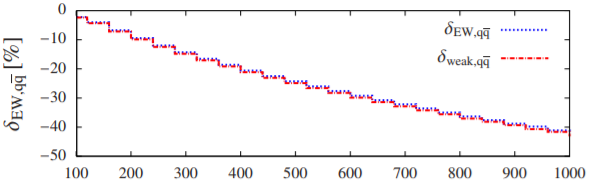
\includegraphics[width=0.49\textwidth]{Figures/Zg_NLO_weights.png}
    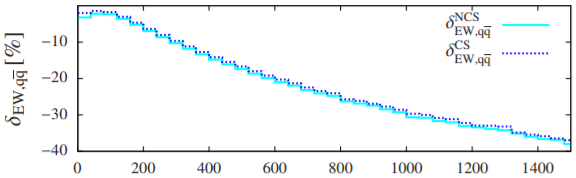
\includegraphics[width=0.49\textwidth]{Figures/Wg_NLO_weights.png}
    \caption{
    Fractional shifts on event weights introduced by NLO EWK corrections, as a function of \pTgamma. Left: \zinvg. Right: \wlng. From~\cite{ref:JHEP04(2015)018, ref:JHEP02(2016)057}.
    }
    \label{fig:NLO_EWK_weights}
  \end{center}
\end{figure}

To avoid numerical divergences that can arise in perturbative calculations, and also to avoid wasting computational cycles simulating events outside the analysis scope of this
thesis, kinematic cuts are applied on the events that may be generated. Most significantly, BSM and $\PW,\PZ + \Pgamma$ events are only simulated if they have a leading
\Pgamma\ with $\pT > 130\unit{GeV}$ emitted within the ECAL acceptance. For consistency, the same generator-level cuts (as well as PDF sets) are applied in both MATRIX and MadGraph.

\section{Parton showering and hadronization} \label{sec:simulation_parton_shower_hadronization}
The output of the hard collision, $X + rest$, continues to evolve as it exits the interaction point.
For example, high-energy quarks and gluons will tend to radiate other high-energy quarks and gluons in a cascading process
known as a parton shower, dispersing their energy as they do so. The energies of the showering partons begin at the hard interaction energy scale
and go down to the hadronization scale (${\lesssim}10\unit{GeV}$). Above this energy scale, $\alpha_\mathrm{S}$ is less than $O(1)$, and so the parton
shower process admits a perturbative analysis in the theory of QCD.
The statistical behavior of parton showering is governed by Sudakov form factors derived from the DGLAP equations~\cite{ref:0034-4885/70/1/R02}.

Below the hadronization scale, the remnant partons will no longer have enough energy to freely split and will finally bind into hadrons
in a process called hadronization. This occurs as the value of $\alpha_\mathrm{S}$ associated with a typical parton energy rises above $O(1)$, rendering estimates
based on perturbative expansions invalid. The bulk of the partons in the colliding protons are not directly involved in the hard parton--parton scatter and are also subject
to a nonperturbative energy scale; these contribute softer showers of particles\footnote{The $rest$ terms in the equations of sec.~\ref{sec:simulation_hard_process}.}
known as the underlying event.
These nonperturbative processes are simulated with generator-dependent phenomenological models, tuned to match the hadronic distributions observed in the experiment.
For all the simulated samples used in this thesis, both parton showering and hadronization are handled by PYTHIA 8.218~\cite{ref:j.cpc.2015.01.024},
with underlying-event tune CUETP8M1~\cite{ref:epjc/s10052-016-3988-x}.

\section{Pileup and detector simulation} \label{sec:simulation_detector}
The simulated contribution from pileup is estimated by overlaying additional ``minimum-bias'' events, with simulated particle distributions
corresponding to the typical \Pp\Pp\ scattering events most likely to occur in the LHC. These are estimated by taking LHC collision data with no
special trigger selections applied. This step of the simulation is also handled by PYTHIA.

The output of the preceding steps is a collection of several thousand stable or semistable particles that continue to propagate outward and interact
with the detector. This stage is handled by GEANT4~\cite{ref:S0168-9002(03)01368-8}, which simulates the decay of long-lived
($0.01\unit{m}/c \lesssim \mathrm{lifetime} \lesssim 10\unit{m}/c$) particles within the detector volume, miscellaneous physical processes including those
discussed in the previous chapter (magnetic bending, electromagnetic showers, hadronic showers, scintillation, etc.), and the response of detector electronics,
leading to the final digitized detector output.

\chapter{Object reconstruction} \label{chap:reconstruction}
\section{The particle-flow algorithm} \label{sec:reconstruction_particle_flow}
The goal of the particle-flow (PF) algorithm is to reconstruct the identities and kinematic properties of all
final-state particles in an event. The CMS is the first hadron collider experiment to have successfully implemented this strategy,
owing to its precise and robust tracking systems, highly granular and hermetic calorimeters, and intense solenoidal magnetic field.
The PF algorithm is described in detail in~\cite{ref:1748-0221/12/10/P10003}.

Particles with lifetimes long enough to exit the beam pipe and reach CMS are divided into six general classes:
electrons, photons, charged hadrons, neutral hadrons, muons, and neutrinos.
Neutrinos do not interact with any of the detector layers, and so PF only attempts to directly reconstruct the other five classes.
Electrons, charged hadrons, and muons leave tracks in the inner tracker, while photons and neutral hadrons do not. Photons and electrons
deposit nearly all their energy in electromagnetic showers in ECAL, which completely stops them from propagating forward to subsequent
detector layers. Generally speaking, hadrons and muons do not produce substantial ECAL showers, and these particles continue on to HCAL.
Hadronic showers usually begin in one of the calorimeters and evolve mainly in HCAL, which fully absorbs them before they can reach the muon detectors.
Muons do not produce hadronic showers and, being MIPs, pass through the inner tracker, calorimeters, solenoid, steel flux-return yoke,
and muon detectors largely unperturbed aside from magnetic bending, leaving tracks in the muon detectors on their way out.
These interactions are illustrated in Fig.~\ref{fig:particle_flow}.

\begin{figure}[hbtp]
  \begin{center}
    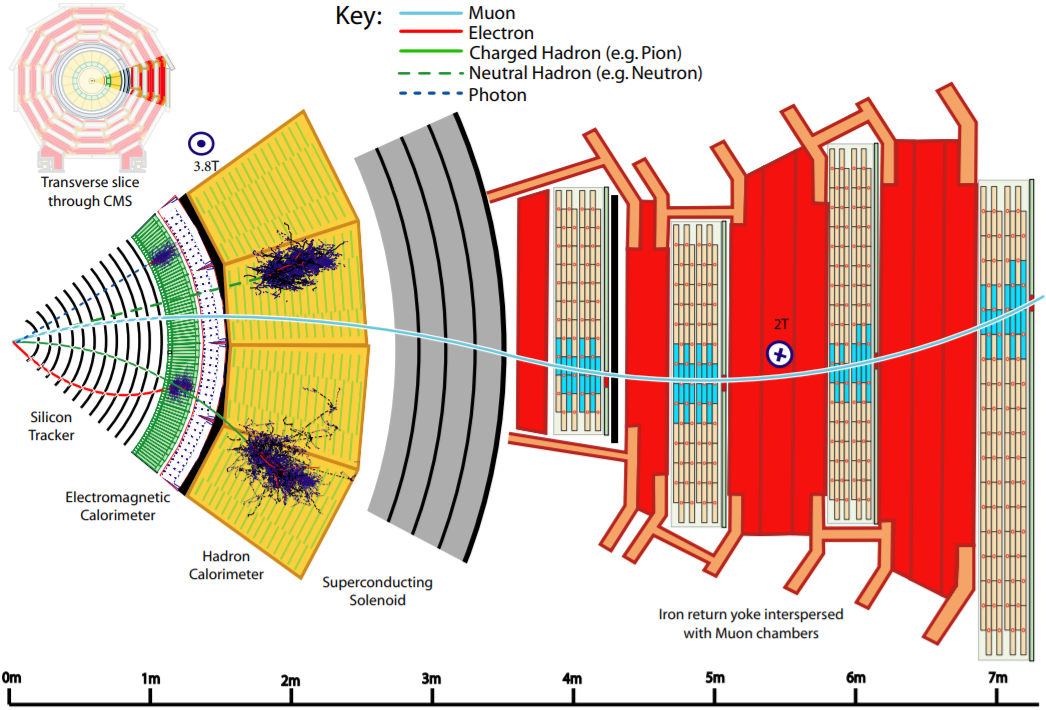
\includegraphics[width=0.99\textwidth]{Figures/particle_flow.png}
    \caption{
    A schematic diagram of CMS overlaid with
    the classes of particles reconstructed by the PF algorithm, showing their most
    characteristic interactions with detector layers.
    From~\cite{ref:1748-0221/12/10/P10003}.
    }
    \label{fig:particle_flow}
  \end{center}
\end{figure}

Each detector layer gives rise to basic characteristic elements used in event reconstruction:
tracks from the inner and muon trackers, and clusters from the ECAL and HCAL. The PF algorithm links these elements together
so as to deduce the species of a particle based on the set of elements present along its trajectory. The linked elements
corresponding to a given particle then provide multiple pieces of data on the particle's behavior, which are synthesized
in order to refine the measurement of the particle's kinematic properties.

Like the physical detector and the trigger apparatus, the reconstruction algorithms employed by CMS are subject to ongoing evolution
and optimization. The details given in this chapter correspond to the specific strategies used in 2016.

\section{Tracks and clusters}
Track reconstruction in the inner tracker is performed over 10 iterations, with the parameters of each iteration tuned to maintain a high selection purity
and reconstruction speed. In each iteration, seeds comprising a few tracker hits are used to initiate an iterative trajectory building algorithm,
which adds a tracker hit to the track according to the Kalman filter method, fits a trajectory to those hits, and then
searches for additional hits compatible with the latest trajectory, until all tracker layers are exhausted~\cite{ref:cms_tdr_vol1}.
Hits assigned to tracks in one iteration are then masked so as to reduce the probability of a misreconstructed track in successive
iterations, allowing the track reconstruction efficiency to grow while simultaneously keeping the purity high.
A separate muon track reconstruction algorithm is seeded by hits in the DTs and CSCs. Hits in the DTs, CSCs, and RPCs are linked along a potential muon trajectory,
resulting in a standalone-muon track.

Clustering is performed separately in EB, EE, HB, HE, and each of the two preshower layers on either endcap\footnote{Separate cells are not clustered in HF.
Rather, each individual HF cell gives rise to one HF EM cluster and one HF HAD cluster, corresponding
to the electromagnetic and hadronic components of each cell, respectively.}. The algorithm proceeds in the same general
fashion in each of these components, with distinct component-dependent threshold values~\cite{ref:1748-0221/12/10/P10003} applied at various steps.
Since this thesis focuses on barrel photons, only EB thresholds are reported here.

An EB crystal is identified as a cluster seed if its energy exceeds 230\unit{MeV} as well as that of its 8 immediate neighbors. Neighboring cells
are progressively added to a topological cluster based on the seed, as long as their energy exceeds 80\unit{MeV} (twice the average noise level in EB)
and they share at least one corner in common with a cell in the cluster. A single topological cluster can grow to encompass multiple seeds.
Once a topological cluster is fully built, the energy distribution in the topological cluster is fit to a sum of Gaussian shapes,
with one Gaussian of width $\sigma = 1.5\unit{cm}$ per seed. Each of the fit shapes then becomes its own cluster, with a position and energy defined by the Gaussian's
mean and amplitude, respectively. In this manner, the energy of a single crystal can be shared between distinct clusters.

A linking algorithm assigns a link between two PF elements if they lie near each other in the $\eta$--$\phi$ plane and satisfy some quality criteria.
Linked elements are then chained together into lattices called blocks. A block corresponding to a simple isolated particle trajectory
may have a simple linear topology, but generic blocks can have treelike structures with various converging and diverging lines.
This reflects the tendency of particles to radiate or decay into other
particles, as well as the possibility that multiple particles may be collimated so closely that their separate contributions to PF elements cannot
reliably be distinguished by just the linking algorithm. Subsequent stages of the PF algorithm identify the particle(s) corresponding to each
block using a sophisticated decision tree. The most robustly-reconstructed particles are identified first and have their contributions to PF elements
subtracted out from those elements, leaving behind residual excesses which can then be identified as other particles.

\section{Photons and electrons} \label{sec:reconstruction_egamma}
Just prior to the installation of ECAL into CMS, the energy resolution of single electrons in the barrel region was estimated
by firing an electron beam directly at the crystal array~\cite{ref:1748-0221/2/04/P04004}.
These measurements show that a $5{\times}5$ crystal array contains about 97\% of an electron shower's energy.
A fit of that data to the functional form\footnote{The symbol ${\oplus}$ denotes addition in quadrature.}
\begin{equation}
\frac{\sigma}{E} = \frac{S}{\sqrt{E}} \oplus \frac{N}{E} \oplus C
\end{equation}
gives $S = 0.028\unit{GeV^{1/2}}$, $N = 0.12\unit{GeV}$, and $C = 0.003$. This indicates that, using
only ECAL shower information, a isolated \Pe\ or unconverted \Pgamma\ with energy around 200\unit{GeV} can have its energy measured to within 0.4\%.

This straightforward picture of a single \Pe\ or \Pgamma\ hitting the ECAL is complicated by the significant depth of tracking material in front of it.
As shown in Fig.~\ref{fig:tracker_thickness}, a minimum of ${\approx}0.4$\,$X_{0}$ of material sits in front of EB, rising up to ${\approx}2$\,$X_{0}$ near $|\eta| = 1.4$.
On average, electrons will radiate away about 33\% of their energy through bremsstrahlung near $|\eta| = 0$, and about 86\% of their energy near $|\eta| = 1.4$~\cite{ref:1748-0221/10/06/P06005}.
The electron trajectory is bent in the $\phi$ coordinate by the solenoid's magnetic field, but the radiated photon trajectories are not, so they are spread widely in $\phi$.
Meanwhile, photons have a substantial chance of converting to an $\Pe^{+}\Pe^{-}$ pair in the tracker. These particles similarly have their trajectories bent in $\phi$ (in opposite directions)
by the magnetic field, and they also radiate photons. The PF algorithm incorporates a dedicated conversion finder~\cite{ref:1748-0221/10/08/P08010} to identify these cases.

\begin{figure}[hbtp]
  \begin{center}
    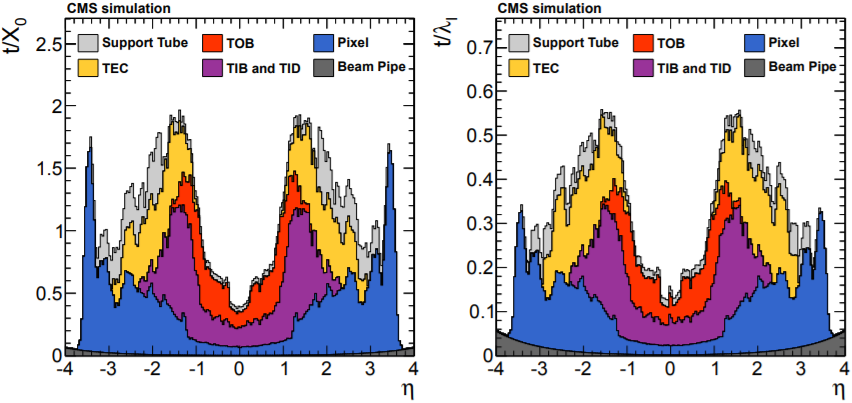
\includegraphics[width=0.90\textwidth]{Figures/tracker_thickness.png}
    \caption{
    Thickness of material in front of ECAL, in multiples of $X_{0}$ (left) and $\lambda_{I}$ (right). From~\cite{ref:1748-0221/9/10/P10009}.
    }
    \label{fig:tracker_thickness}
  \end{center}
\end{figure}

Bremsstrahlung photons tend to emerge nearly parallel to the parent electron's motion, and so have momentum vectors lying tangent to the electron's track.
As part of the linking algorithm, tangent lines from the track are drawn at each of its intersections with the tracker layers. If one of these tangent lines,
extrapolated forward, is compatible with the position of an ECAL cluster (or a conversion track pair identified by the conversion finder), the cluster (or track pair)
is linked to the track as a possible bremsstrahlung photon.

Any energy recorded in the preshower detector is added to that of the closest ECAL cluster (or else discarded if no associated cluster is found).

A ``Swiss cross'' cut is applied in order to reject spikes:
defining $E_{1}$ to be the energy of the seed crystal and $E_{4}$ to be the sum of the energies of the 4 neighboring crystals,
a PF photon is only reconstructed if $E_{4}/E_{1} > 0.05$. Double spikes are suppressed by a similar cut based on the ratio of $E_{2}$, the sum of the energies
of the seed crystal and its highest-energy neighbor, and $E_{6}$, the sum of the energies of the six neighboring crystals surrounding the first
two. Further spike rejection is achieved by requiring the time of energy deposits above 1\unit{GeV} to be within 2\unit{ns} of the bunch crossing time.

The response of calorimeter cells is periodically calibrated so as to faithfully reproduce the shower energy they contain.
Due to the thresholds imposed in the clustering stage, some of this energy will tend to be left out of PF clusters, and therefore another
layer of calibrations is applied to these clusters in order to restore this energy. Bremsstrahlung and photon conversions introduce multiple
additional particles to the event, with multiple opportunities for energy to be lost as particles escape through small cracks in the detector, fall into dead
regions, etc. Thus, a third layer of particle-specific calibrations is derived for photons and electrons. The energy most commonly reported in
CMS analyses is this final calibrated value.

Photons typically have their energies raised by up to a few percent by the last set of calibrations. However, after examining monophoton events with
probable non-photon objects misreconstructed as photons, we have determined that these ``fake'' photons are often assigned very large energy shifts
on the order of 100\%, badly skewing their energies upward. This is due to the fact that fake photons tend to have atypical photon shower shapes,
and the calibrations, based on simulated ``real'' photon events, were derived as a function of shower shape\footnote{For this reason, calibrations
derived in 2017 and 2018 are independent of shower shape~\cite{ref:egammaclusterregression_2018}.}.
High-\ETgamma\ events have the least precisely measured cross sections, and are also the most sensitive probes of the BSM models examined in this thesis.
In order to minimize contamination of this sensitive kinematic region, we have opted to use the uncalibrated ``raw''
photon supercluster \ET\ as the reconstructed quantity in which to bin our data.

\section{Muons} \label{sec:reconstruction_muons}
A track in the inner tracker qualifies as a tracker-muon track if its extrapolated trajectory matches at least one hit in the muon systems.
If an inner track fits together with a standalone-muon track, hits in both tracks are fit to a common global-muon track.
About 99\% of muons produced within the $\eta$ coverage of the muon systems are reconstructed as a global or tracker muon\footnote{They are often reconstructed
as both. A separate global muon and tracker muon are merged into a single muon candidate if they share the same inner track.}.
The additional hit data markedly improves the momentum resolution of muons with $\pT \gtrsim 200\unit{GeV}$~\cite{ref:1748-0221/12/10/P10003}.

A muon candidate is accepted as an isolated muon if the tracks and calorimeter deposits within $\Delta R < 0.3$ of the candidate muon have a total \pT\ no greater than 10\%
of the candidate muon \pT. A muon that fails this criterion can still be accepted as a nonisolated muon if it passes a ``tight'' muon ID, as defined in~\cite{}.
It can also be accepted if it has a high-quality global or inner track with a large number of hits, as long as any associated calorimeter clusters are compatible with the muon hypothesis.

Once a muon is accepted, its \pT\ is derived from its track. For high-\pT\ (${>}200\unit{GeV}$) candidates, 

\section{Jets and missing transverse momentum} \label{sec:reconstruction_jetmet}
As a consequence of parton showering and hadronization, a single radiated quark or gluon from a hard-scatter event does not reach the CMS detector
as a single particle, but rather a collimated ``jet'' of hadrons (mostly pions) and their decay products (such as photons from neutral pion decays).
The goal of a jet reconstruction algorithm is to identify which final-state particles arose in such a manner, group them according to their originating
particle, and recover as accurately as possible the properties of the that particle.

The output of the PF algorithm is a set of basic particles of the five types described above. These serve as the input to the anti-kT algorithm

Discussion of jets is followed by a definition of \MET\ and Type-1 \MET\ corrections.

\chapter{Event selection} \label{chap:event_selection}
\section{The monophoton signature and background sources} \label{sec:event_selection_backgrounds}
Summarize how each of the physics processes being analyzed exhibits a monophoton signature.
List the sources of background in the monophoton channel, to justify the ensuing cuts.
\section{Trigger and \texorpdfstring{\MET}{pTmiss} filters} \label{sec:event_selection_trigger_METfilters}
Trigger path, trigger efficiency

\MET\ filters
\section{Photon} \label{sec:event_selection_photon}
Photon kinematic cuts; Photon ID defintion, efficiency; Spike and beam halo cuts; phoET-dependent cross section corrections
% Pixel seed defined in ref:1748-0221/10/08/P08010

\section{Missing transverse momentum} \label{sec:event_selection_MET}
$\MET > 170$ GeV; $\Delta\phi(\Pgamma,\vecMET) > 0.5$; $\mathrm{min}\Delta\phi(\mathrm{jets},\vecMET) > 0.5$;
$\ETgamma/\MET < 1.4$
\section{Lepton vetoes} \label{sec:event_selection_lepveto}
Electron selection; Muon selection
\section{Single electron control region} \label{sec:event_selection_monoele}
\section{Single muon control region} \label{sec:event_selection_monomu}
\section{Dielectron control region} \label{sec:event_selection_diele}
\section{Dimuon control region} \label{sec:event_selection_dimu}

\chapter{Background estimation} \label{chap:background_estimation}
For each component, describe its estimation and uncertainties
\section{Simulated backgrounds} \label{sec:background_estimation_simulated}
\section{Electron faking photon} \label{sec:background_estimation_elefake}
\section{Jet faking photon} \label{sec:background_estimation_jetfake}
\section{Spikes} \label{sec:background_estimation_spikes}
\section{Beam halo} \label{sec:background_estimation_halo}
\section{Transfer factors} \label{sec:background_estimation_transfer_factors}
\section{Likelihood function} \label{sec:background_estimation_likelihood}

\chapter{Results} \label{chap:results}
\section{\texorpdfstring{\zinvg}{Z(νν)γ} cross section} \label{sec:results_znng_xsec}
\section{aTGC limits} \label{sec:results_aTGC}
\section{DM simplified model limits} \label{sec:results_DM}
\section{ADD limits} \label{sec:results_ADD}

\chapter{Conclusions} \label{chap:conclusions}
\section{Summary} \label{sec:conclusions_summary}
\section{Outlook} \label{sec:conclusions_outlook}

\bibliographystyle{utcaps}
\bibliography{references}
\end{document}
